% VerA.web-Installationsanleitung
%
% Copyright © 2015, 2016, 2017, 2018, 2019, 2020
%	Thorsten Glaser <t.glaser@tarent.de>
% Copyright © 2014, 2015
%	Thorsten Glaser <thorsten.glaser@teckids.org>
% Copyright © 2013, 2014
%	Dominik George <dominik.george@teckids.org>
%
% Contains excerpts of configuration files licenced to the ASF under
% one or more contributor license agreements and published under the
% Apache License, Version 2.0 — see the global VerA.web LICENCE file
% for details, terms and the “NOTICE” file contents.
%
% Provided that these terms and disclaimer and all copyright notices
% are retained or reproduced in an accompanying document, permission
% is granted to deal in this work without restriction, including un‐
% limited rights to use, publicly perform, distribute, sell, modify,
% merge, give away, or sublicence.
%
% This work is provided “AS IS” and WITHOUT WARRANTY of any kind, to
% the utmost extent permitted by applicable law, neither express nor
% implied; without malicious intent or gross negligence. In no event
% may a licensor, author or contributor be held liable for indirect,
% direct, other damage, loss, or other issues arising in any way out
% of dealing in the work, even if advised of the possibility of such
% damage or existence of a defect, except proven that it results out
% of said person’s immediate fault when using the work as intended.
%-
% Characters requiring escaping:
% • { } # & _ % $ ⇒ quote by prepending a backslash \
% • \ → \textbackslash
% • ^ → \textasciicircum
% • ~ → \textasciitilde
% • (nbsp) → ~
% • (em dash) → \dash

\documentclass{tarentanleitung}
\usepackage{tikz}
\usetikzlibrary{arrows,backgrounds,fit,positioning,shapes,shadows}
\lstset{moredelim=[is][\color{RoyalPurple}]{【}{】}}%

% VerA.web Fassung der Installationsanleitung
\newcommand{\vwiaversfassungnr}{7.7}
\newcommand{\vwiaversfassungmonat}{May}
\newcommand{\vwiaversfassungjahr}{2020}

% VerA.web Version
\newcommand{\vwiaverssw}{2.3}

\begin{document}
\tarentanleitung{Installationsanleitung VerA.web}{\vwiaverssw}
 {\vwiaversfassungnr}{\vwiaversfassungmonat}{\vwiaversfassungjahr}{veraweblogo}

% uncomment if this is a WIP that should not be published
%\fancyfoot[RO,LE]{\leavevmode\usekomafont{pageheadfoot}⚠ Work in Progress, do not use}

% LaTeX Table of Contents for tarent
%
% Copyright © 2015
%	Thorsten Glaser <t.glaser@tarent.de>
%
% Provided that these terms and disclaimer and all copyright notices
% are retained or reproduced in an accompanying document, permission
% is granted to deal in this work without restriction, including un‐
% limited rights to use, publicly perform, distribute, sell, modify,
% merge, give away, or sublicence.
%
% This work is provided “AS IS” and WITHOUT WARRANTY of any kind, to
% the utmost extent permitted by applicable law, neither express nor
% implied; without malicious intent or gross negligence. In no event
% may a licensor, author or contributor be held liable for indirect,
% direct, other damage, loss, or other issues arising in any way out
% of dealing in the work, even if advised of the possibility of such
% damage or existence of a defect, except proven that it results out
% of said person’s immediate fault when using the work as intended.
%-
% include with 「% LaTeX Table of Contents for tarent
%
% Copyright © 2015
%	Thorsten Glaser <t.glaser@tarent.de>
%
% Provided that these terms and disclaimer and all copyright notices
% are retained or reproduced in an accompanying document, permission
% is granted to deal in this work without restriction, including un‐
% limited rights to use, publicly perform, distribute, sell, modify,
% merge, give away, or sublicence.
%
% This work is provided “AS IS” and WITHOUT WARRANTY of any kind, to
% the utmost extent permitted by applicable law, neither express nor
% implied; without malicious intent or gross negligence. In no event
% may a licensor, author or contributor be held liable for indirect,
% direct, other damage, loss, or other issues arising in any way out
% of dealing in the work, even if advised of the possibility of such
% damage or existence of a defect, except proven that it results out
% of said person’s immediate fault when using the work as intended.
%-
% include with 「% LaTeX Table of Contents for tarent
%
% Copyright © 2015
%	Thorsten Glaser <t.glaser@tarent.de>
%
% Provided that these terms and disclaimer and all copyright notices
% are retained or reproduced in an accompanying document, permission
% is granted to deal in this work without restriction, including un‐
% limited rights to use, publicly perform, distribute, sell, modify,
% merge, give away, or sublicence.
%
% This work is provided “AS IS” and WITHOUT WARRANTY of any kind, to
% the utmost extent permitted by applicable law, neither express nor
% implied; without malicious intent or gross negligence. In no event
% may a licensor, author or contributor be held liable for indirect,
% direct, other damage, loss, or other issues arising in any way out
% of dealing in the work, even if advised of the possibility of such
% damage or existence of a defect, except proven that it results out
% of said person’s immediate fault when using the work as intended.
%-
% include with 「\input{toc.tex}」 after \tarentanleitung{…}…

\addtocontents{toc}{\protect\thispagestyle{fancy}}
\addtolength{\cftsubsecnumwidth}{0.5em}
\addtolength{\cftsubsubsecindent}{0.5em}
\renewcommand{\cftsecleader}{\cftdotfill{\cftdotsep}}
\hypersetup{linkcolor = black}
\tableofcontents
\hypersetup{linkcolor = blue}
\newpage
」 after \tarentanleitung{…}…

\addtocontents{toc}{\protect\thispagestyle{fancy}}
\addtolength{\cftsubsecnumwidth}{0.5em}
\addtolength{\cftsubsubsecindent}{0.5em}
\renewcommand{\cftsecleader}{\cftdotfill{\cftdotsep}}
\hypersetup{linkcolor = black}
\tableofcontents
\hypersetup{linkcolor = blue}
\newpage
」 after \tarentanleitung{…}…

\addtocontents{toc}{\protect\thispagestyle{fancy}}
\addtolength{\cftsubsecnumwidth}{0.5em}
\addtolength{\cftsubsubsecindent}{0.5em}
\renewcommand{\cftsecleader}{\cftdotfill{\cftdotsep}}
\hypersetup{linkcolor = black}
\tableofcontents
\hypersetup{linkcolor = blue}
\newpage


\section{Einleitung}\label{sec:intro}

„VerA.web“ steht für Veranstaltungs‑ und Adreßverwaltung im „web“ (Internet).
VerA.web ist eine Open Source-Webanwendung, die die IT-gestützte Planung und
Durchführung von Anlässen, Konferenzen und anderen Veranstaltungen maßgeblich
unterstützt.

\subsection{Über diese Anleitung}\label{subsec:aboutmanual}

Dieses Dokument beschreibt, wie das Veranstaltungsmanagement
VerA.web durch einen Systemadministrator
eigenständig installiert werden kann. Hierbei wird eine empfohlene
Installation beschrieben; ein Betrieb ist auch mit abweichender
Konfiguration (z.B. ohne Apache) möglich, aber nicht durch dieses
Dokument abgedeckt.

Diese Anwendung verwendet blau gedruckte Verweise auf andere Kapitel,
z.B. über den Kapitelnamen (Beispiel: \nameref{subsec:aboutmanual})
oder über die Kapitelnummer (Beispiel: \ref{subsec:aboutmanual});
beide Beispiele verweisen auf den aktuellen Abschnitt. Einige Links
gehen auf externe Ressourcen (z.B. die \tarent{}-Webseite,
das Benutzerhandbuch). Wenn Sie diese Anleitung als
PDF am Computer lesen sind die Links (inklusive der schwarz gedruckten
Einträge im Inhaltsverzeichnis) folgbar; in der Druckversion schauen
Sie bitte ggfs. die Seite des Kapitels im Inhaltsverzeichnis nach.

\subsubsection{Listings}\label{subsubsec:aboutmanual-lst}

\begin{minipage}{\linewidth}
Alle Code-Listings finden Sie auch nochmal als Plaintext unter
\texttt{\jobname.lst} im „files“-Tarball
(\texttt{veraweb-core-\vwiaverssw{}-files.tgz}, siehe
\nameref{subsec:intro-distro}).
Zwecks Zuordnung finden Sie die Listing-Nummern am äußeren
Seitenrand bzw. als Teil der Überschrift in der Listing-Datei.

\begin{lstdumpx}
Dies ist beispielsweise Listing 1.
\end{lstdumpx}
\end{minipage}

\subsubsection{Annahmen}\label{subsubsec:aboutmanual-assume}

Die Installation von VerA.web ist äußerst flexibel und anpaßbar.
In dieser Anleitung haben wir daher einige Annahmen getroffen, um
sie nicht wegen kombinatorischer Explosion der Möglichkeiten noch
unverständlicher zu machen. Hierzu gehören:\keinumbruch

\begin{itemize}
 \item{Die Installation wird auf nicht anderweitig verwendeten,
  sauberen oder frisch installierten (virtuellen) Maschinen durchgeführt.}
 \item{Als Betriebssystem wird Debian~9 „stretch“ eingesetzt; an den
  Stellen, wo Konfigurationsdateien angepaßt werden müssen, werden die
  Debian-Standardwerte als Grundlage vorausgesetzt. \texttt{sudo} ist
  installiert und eingerichtet.}
 \item{⚠ Aktuell wird eine Debian-Installation mit \texttt{sysvinit},
  \emph{nicht} \texttt{systemd}, vorausgesetzt!}
 \item{Das System ist grundsätzlich installiert, betriebsbereit
  und rebootfest; Firewalleinstellungen sind hinreichend getroffen.
  Für jede Maschine ist ein gültiges SSL-Zertifikat vorhanden, das
  alle verwendeten Hostnamen abdeckt.}
 \item{Die PostgreSQL-Datenbank für VerA.web wird auf dem System
  lokal installiert. (Abweichungen sind trivial möglich.)
  Die REST-API wird nicht vom VerA.web core getrennt.}
\end{itemize}

\subsection{Konzepte}\label{subsec:concepts}

Der Kern von VerA.web besteht aus zwei Webanwendungen, die in einem
Java-Applikationsserver (Apache Tomcat) laufen. Diese beiden Komponenten
werden in der Regel auf demselben Server installiert und greifen auf
dieselbe Datenbank zu.

\begin{itemize}
 \item{\texttt{veraweb.war}: Die eigentliche Veranstaltungsmanagementsoftware,
  welche später über einen Apache-Webserver von Sachbearbeitern bedient wird.}
 \item{\texttt{vwor.war}: Ein Hilfsmodul, welches intern angesprochen wird.}
\end{itemize}

VerA.web authentifiziert Sachbearbeiter über einen \nameref{subsec:req-ldap}.
Ein LDAP-Server ist Voraussetzung für den Betrieb von VerA.web.
(Falls Sie keinen LDAP-Server betreiben können Sie anhand dieser Anleitung
einen schlanken LDAP-Server mit Administrations-Webfrontend aufsetzen.)

Es wird grundsätzlich (insbesondere mit Blick auf das BDSG und die EU-DSGVO)
empfohlen, nur mit der Administration der Systeme betreuten Personen Zugriff
auf die Systeme auf Shell-Ebene zu gewähren, und weitere geeignete Maßnahmen
zur Absicherung der Gesamtinstallation und aller Komponenten zu treffen.
Diese sprengen jedoch den Rahmen dieses Dokuments.

\subsection{Systemübersicht}\label{subsec:intro-overview-blocks}

Im folgenden finden Sie eine grobe Übersicht über die einzelnen oben
erwähnten Komponenten und ihr Zusammenspiel:\keinumbruch

\begin{minipage}{\linewidth}
\vspace{5mm}
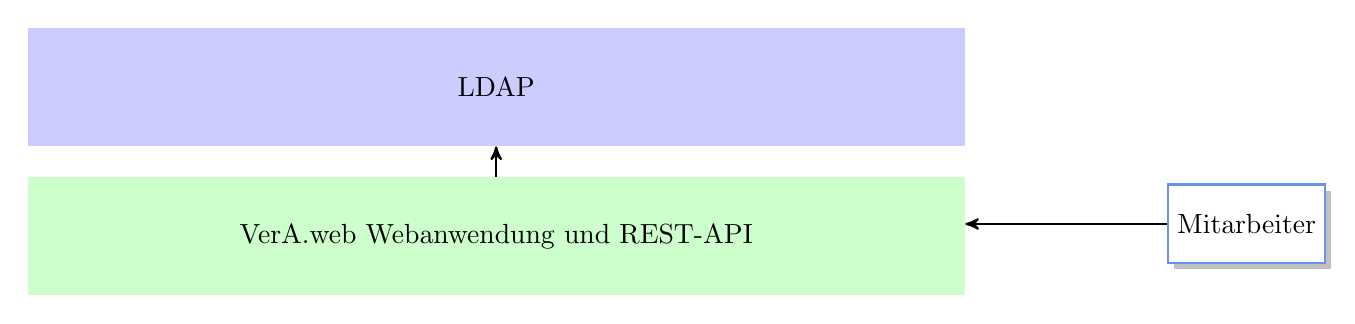
\begin{tikzpicture}[
  >=stealth',
  people/.style={thick,text=black,fill=white,drop shadow,minimum height=10mm,above left,rectangle,draw=CornflowerBlue,minimum width=12mm},
 ]

  \node[above right,rectangle,fill=blue!20,minimum width=119mm,minimum height=15mm] (ldap) at (3mm,23mm) {LDAP};
  \node[above right,rectangle,fill=green!20,minimum width=119mm,minimum height=15mm] (web) at (3mm,4mm) {VerA.web Webanwendung und REST-API};

  \node[people]   (sb)     at (168mm,8mm) {Mitarbeiter};

  \draw[thick,->] (web) -- (ldap);
  \draw[thick,->] (sb.west) -- (sb-|web.east);

\end{tikzpicture}
\end{minipage}

\subsection{Die Rolle der REST-API}\label{subsec:intro-restapi}

Die Aufrufe der REST-API werden durch HTTP Basic Authentication mit einem
(Maschinen‑)Benutzernamen und Paßwort gesichert, welche bei der aufrufenden
Kernanwendung hinterlegt wird; die REST-API wird niemals direkt durch
einen Menschen bedient. Es wird standardmäßig der Benutzer \texttt{veraweb}
mit dem Paßwort \texttt{veraweb} verwendet; eine Änderung der Zugangsdaten
ist \emph{dringend empfohlen}, um die Betriebssicherheit zu gewährleisten;
an den entsprechenden Stellen in dieser Anleitung finden Sie Hinweise hierzu.

\subsection{Detailübersicht}\label{subsec:intro-overview-coarse}

In der nächsten Graphik werden die zur Installation von VerA.web
gehörenden Komponenten mit mehr Detailtiefe aufgeschlüsselt:\keinumbruch

\begin{minipage}{\linewidth}

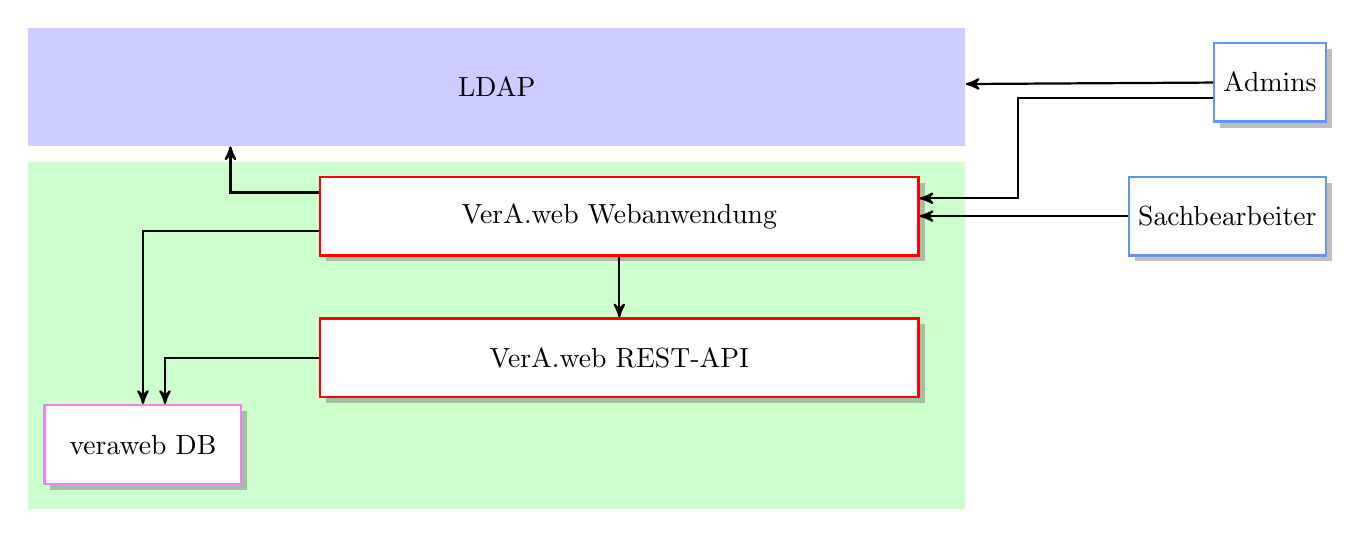
\begin{tikzpicture}[
  >=stealth',
  microsvc/.style={thick,text=black,fill=white,drop shadow,minimum height=10mm,above right,rectangle,draw=Orange,minimum width=76mm},
  webapp/.style={thick,text=black,fill=white,drop shadow,minimum height=10mm,above right,rectangle,draw=red,minimum width=76mm},
  syssvc/.style={thick,text=black,fill=white,drop shadow,minimum height=10mm,above right,rectangle,draw=Violet,minimum width=25mm},
  scrptr/.style={thick,text=black,fill=white,drop shadow,minimum height=10mm,above right,rectangle,draw=black,minimum width=25mm},
  scrptl/.style={thick,text=black,fill=white,drop shadow,minimum height=10mm,above left,rectangle,draw=black,minimum width=25mm},
  people/.style={thick,text=black,fill=white,drop shadow,minimum height=10mm,above left,rectangle,draw=CornflowerBlue,minimum width=12mm},
 ]

% \draw (0mm,0mm) -- (0mm,120mm) -- (173mm,120mm) -- (173mm,0mm) -- (0mm,0mm);

  \fill[green!20] (2mm,50mm) -- (121mm,50mm) -- (121mm,94mm) -- (2mm,94mm);

  \node[above right,rectangle,fill=blue!20,minimum width=119mm,minimum height=15mm] (ldap) at (2mm,96mm) {LDAP};

  \node[webapp]   (score)  at ( 39mm,82mm) {VerA.web Webanwendung};
  \node[webapp]   (svwor)  at ( 39mm,64mm) {VerA.web REST-API};
  \node[syssvc]   (dbvw)   at (  4mm,53mm) {veraweb DB};
  \node[people]   (admins) at (167mm,99mm) {Admins};
  \node[people]   (sb)     at (167mm,82mm) {Sachbearbeiter};

  \draw[thick,->] (admins) -- ([yshift=3mm]ldap);
  \draw[thick,->] ([yshift=-9mm]admins) -| +(-32mm,0mm) |- ([yshift=3mm]score);
  \draw[thick,->] ([yshift=3mm]score.west) -| ([xshift=-60mm]ldap);
  \draw[thick,->] (sb) -- (score);
  \draw[thick,->] ([yshift=-3mm]score) -| (dbvw);
  \draw[thick,->] (score.south) -- (score|-svwor.north);
  \draw[thick,->] (svwor) -| ([xshift=6mm]dbvw);

\end{tikzpicture}

\end{minipage}

Auch in dieser Abbildung wird LDAP zur Vereinfachung als Blackbox dargestellt.

\subsection{Apache als Frontend}\label{subsec:intro-apache}

Wir empfehlen üblicherweise, alle Systeme aus Sicherheitsgründen so
aufzusetzen, daß HTTPS-Verbindungen im Apache Webserver terminiert
werden und von diesem an die einzelnen Anwendungsserver (über das
AJP-Protokoll an Tomcat) weitergereicht werden. Sämtliche SSL/TLS-Keys,
‑Features und weitere sicherheitsrelevante Einstellungen werden im
Apache Webserver eingerichtet, auch um die Angriffsoberfläche zu reduzieren
und besser getesteten und weiter verbreiteten Code zu verwenden, und weil
die Administration der genannten Features in Apache bekannter und erprobter
ist als in den individuellen Anwendungsservern. Sie \emph{können} die
Dienste auch direkt über HTTP ansprechen oder SSL in Java terminieren,
dies widerspricht jedoch unserem empfohlenen Setup und kann nicht, z.B.
im Rahmen dieser Anleitung, unterstützt werden.

Es wird je eine Installation des Webservers pro VM benötigt, da in
der von uns empfohlenen Installationsmethode die Komponenten auch
untereinander ausschließlich verschlüsselt und sicher über HTTPS
miteinander kommunizieren.

\subsection{Komponentendiagramm}\label{subsec:intro-overview-fine}

In dieser Darstellung schlüsseln wir die verwendeten Komponenten
detailliert auf. In der linken Spalte finden Sie Systemdienste
(LDAP, Mailserver) und PostgreSQL-Datenbanken, in der zweiten
Spalte finden Sie die eigentlichen Dienste, in der dritten Spalte
die zugehörigen Apache-Frontends, und in der vierten Spalte die
Benutzer. In schwarzen Kästen befinden sich jeweils zugehörige
Skripte.

\begin{minipage}{\linewidth}

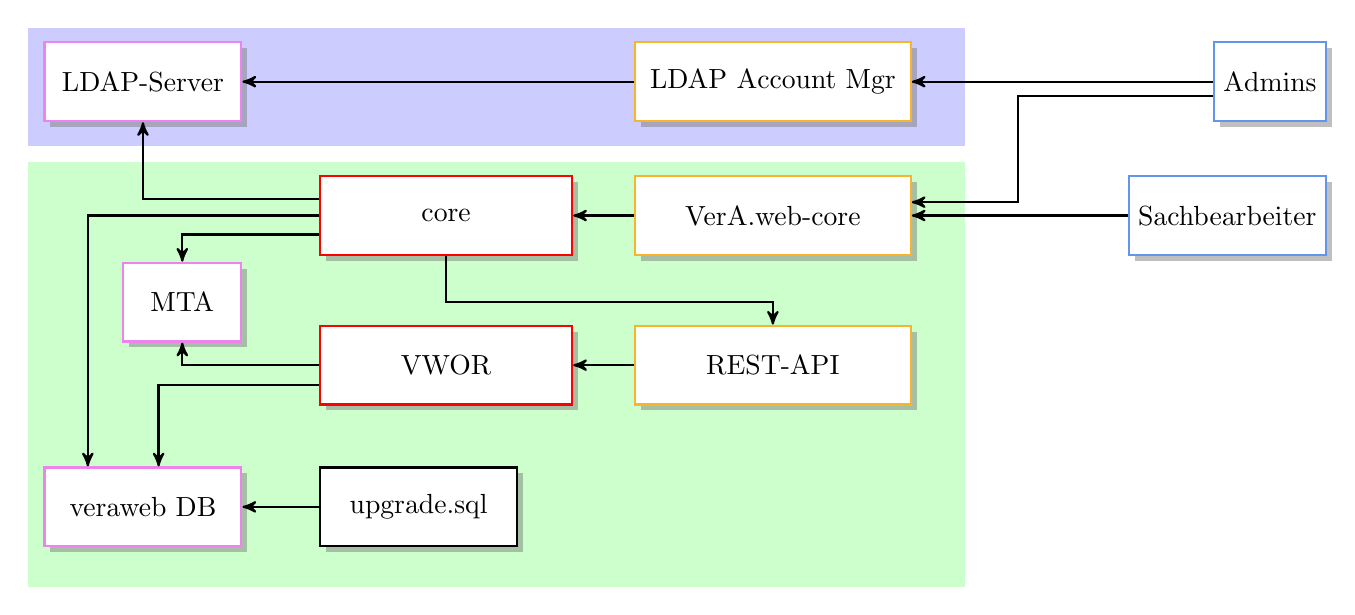
\begin{tikzpicture}[
  >=stealth',
  every node/.style={thick,text=black,fill=white,drop shadow},
  every rectangle node/.style={minimum height=10mm},
  apache/.style={above right,rectangle,draw=Dandelion,minimum width=35mm},
  microsvc/.style={above right,rectangle,draw=Orange,minimum width=32mm},
  webapp/.style={above right,rectangle,draw=red,minimum width=32mm},
  syssvc/.style={above right,rectangle,draw=Violet,minimum width=25mm},
  sysmta/.style={above right,rectangle,draw=Violet,minimum width=15mm},
  scrptr/.style={above right,rectangle,draw=black,minimum width=25mm},
  scrptl/.style={above left,rectangle,draw=black,minimum width=25mm},
  people/.style={above left,rectangle,draw=CornflowerBlue,minimum width=12mm},
 ]

% \draw (0mm,0mm) -- (0mm,120mm) -- (173mm,120mm) -- (173mm,0mm) -- (0mm,0mm);

  \fill[green!20] (2mm,40mm) -- (121mm,40mm) -- (121mm,94mm) -- (2mm,94mm);
  \fill[blue!20] (2mm,96mm) -- (121mm,96mm) -- (121mm,111mm) -- (2mm,111mm);

  \node[apache]   (alam)   at ( 79mm,99mm) {LDAP Account Mgr};
  \node[apache]   (acore)  at ( 79mm,82mm) {VerA.web-core};
  \node[apache]   (avwor)  at ( 79mm,63mm) {REST-API};
  \node[webapp]   (score)  at ( 39mm,82mm) {core};
  \node[webapp]   (svwor)  at ( 39mm,63mm) {VWOR};
  \node[syssvc]   (ldap)   at (  4mm,99mm) {LDAP-Server};
  \node[syssvc]   (dbvw)   at (  4mm,45mm) {veraweb DB};
  \node[sysmta]   (mta)    at ( 14mm,71mm) {MTA};
  \node[scrptr]   (usql)   at ( 39mm,45mm) {upgrade.sql};
  \node[people]   (admins) at (167mm,99mm) {Admins};
  \node[people]   (sb)     at (167mm,82mm) {Sachbearbeiter};

  \draw[thick,->] (admins) -- ([yshift=3mm]alam);
  \draw[thick,->] (alam) -- (ldap);
  \draw[thick,->] ([yshift=-8mm]admins) -| +(-32mm,0mm) |- ([yshift=3mm]acore);
  \draw[thick,->] (acore) -- (score);
  \draw[thick,->] ([yshift=5mm]score) -| (ldap);
  \draw[thick,->] (sb) -- (acore);
  \draw[thick,->] (score) -| ([xshift=-7mm]dbvw.north);
  \draw[thick,->] ([yshift=-5mm]score) -| (mta);
  \draw[thick,->] (svwor) -| (mta);
  \draw[thick,->] (score) |- +(25mm,-11mm) -| (avwor);
  \draw[thick,->] (avwor) -- (svwor);
  \draw[thick,->] ([yshift=-5mm]svwor) -| ([xshift=6mm]dbvw);
  \draw[thick,->] (usql) -- (dbvw);

\end{tikzpicture}

\vspace{0.3cm}

\begin{tabu} to \linewidth {rllll}
\rowfont\bfseries\multicolumn{5}{c}{Legende}\\[0.2cm]
 Erste Spalte: & \multicolumn{4}{l}{%
			\tikz \node[thick,rectangle,draw=Violet] {};
			Systemdienst (LDAP, Mailserver,
			PostgreSQL-Datenbank)}\\
Zweite Spalte: & \multicolumn{2}{l}{%
			\tikz \node[thick,rectangle,draw=red] {};
			Webservice (WAR) in Tomcat} &
		 \multicolumn{2}{l}{%
			\tikz \node[thick,rectangle,draw=black] {};
			Skript (Installation/Upgrade)}\\
Dritte Spalte: & \multicolumn{4}{l}{%
			\tikz \node[thick,rectangle,draw=Dandelion] {};
			 Apache Webserver (SSL, mod\_jk)}\\
Vierte Spalte: & \multicolumn{2}{l}{%
			\tikz \node[thick,rectangle,draw=CornflowerBlue] {};
			 Nutzergruppe (per Webbrowser)} &
		 \multicolumn{2}{l}{}\\
 Schattierung: & \tikz \node[rectangle,fill=blue!30] {}; LDAP &
		 \tikz \node[rectangle,fill=green!30] {}; VerA.web core &
		 &
		 \\
\end{tabu}

\end{minipage}

Die WAR‑ und JAR-Dateien aus der zweiten Spalte finden Sie im
nächsten Abschnitt als individuelle Einträge. Die schwarz
umrahmten Skripte befinden sich im \texttt{files}-Tarball.

\subsection{Die VerA.web-Distribution}\label{subsec:intro-distro}

Zur Installation bzw. Upgrade müssen Sie folgende Dateien („die
VerA.web-Distribution“) von tarent beziehen:\keinumbruch

\begin{itemize}
 \item{\texttt{veraweb-core-\vwiaverssw{}-files.tgz}}
 \item{\texttt{veraweb-core-\vwiaverssw{}.war}}
 \item{\texttt{rest-api-\vwiaverssw{}.war}}
\end{itemize}

Bitte wenden Sie sich hierzu an unseren Produktvertrieb.

\subsection{Installationsvorgehen}\label{subsec:intro-install}

Installation und Upgrade von VerA.web funktionieren, indem
zunächst Teile der Distribution (siehe oben) auf den Server
kopiert werden, und alle weiteren Schritte dann auf dem System
stattfinden. Die Beispiele sind so gehalten, daß die gesamte
Installation als normaler Benutzer oder \texttt{root} auf dem
jeweiligen
Server durchgeführt werden kann, und privilegierte Operationen
mit Hilfe des Programms \texttt{sudo} durchgeführt werden.

Die weiteren Schritte, die auf dem Server durchzuführen sind,
involvieren:\keinumbruch

\begin{itemize}
 \item{Entpacken des \texttt{files}-Tarballs}
 \item{Wechseln in ein spezifisches Unterverzeichnis \dash
  alle weiteren Schritte nehmen an, daß dieses Unterverzeichnis
  Ihr aktuelles Arbeitsverzeichnis ist; sollten Sie zwischendurch
  das Verzeichnis wechseln müssen, wechseln Sie einfach zurück,
  bevor Sie den jeweils nächsten Schritt angehen.}
 \item{Anpassen von (Konfigurations‑)Dateien}
 \item{Installation von Dateien und Neustart von Diensten}
 \item{Löschen der ausgepackten Dateien und Installationsarchive}
\end{itemize}

Bei einem Upgrade möchten Sie ggfs. vorher eine Sicherung erstellen.

\subsection{Exkurs: Wechsel von systemd nach sysvinit}\label{subsec:intro-sysvinit}

Eine Standardinstallation (kein Upgrade) von Debian~8 „jessie“ oder neuer
benutzt \texttt{systemd} als Init-System. Wir haben unsere Software jedoch
ausschließlich mit \texttt{sysvinit}, das Unix-Administratoren vertrauter
ist, getestet.

\begin{minipage}{\linewidth}
Zum Wechsel führen Sie folgenden Befehl aus:

\begin{lstdump}{sysvinit installieren}
sudo apt-get install sysvinit-core
\end{lstdump}

Danach rebooten Sie das System. Prüfen Sie dann, welches \texttt{init} läuft:

\begin{lstdump}{init herausfinden}
sudo ls -l /proc/1/exe
\end{lstdump}

Wenn hinter dem „Pfeil“ \texttt{->} in der Ausgabe der Text
\texttt{/lib/systemd/systemd} steht war der Vorgang nicht
erfolgreich; bei \texttt{/sbin/init} stimmt alles, und Sie
können, falls Sie möchten (dies ist nicht zur Benutzung von
VerA.web notwendig), nun \texttt{systemd} ganz entfernen:

\begin{lstdump}{systemd entfernen}
sudo apt-get purge --auto-remove systemd
\end{lstdump}
\end{minipage}

Einer Nutzung von VerA.web unter \texttt{systemd} steht
nichts Grundsätzliches im Wege; es sprengt lediglich den
aktuellen Rahmen dieser Anleitung und erschwert die
Nutzung von daemontools.

\section{Systemvoraussetzungen}\label{sec:requirements}

In der Angabe für den benötigten Festplattenplatz ist die
Grundinstallation des Betriebssystems (ohne Auslagerungsdatei)
einkalkuliert.

\begin{tabu} to \linewidth {|X[r]||l|l|l|}\hline
                          & Minimum                & empfohlen     & Maximum\\\hline\hline
 Anzahl Prozessoren je VM & 1                      & 1             & 1\Hair\textsuperscript{\ref{fn:req-tst-notmore}}\\\hline
 Betriebssystem           & Debian 8 („jessie“)    & 9 („stretch“) & 9 („stretch“)\Hair\textsuperscript{\ref{fn:req-notmore}}\\\hline
 Java™-Laufzeitumgebung   & OpenJDK 8 JRE headless & wie Minimum   & OpenJDK 11\Hair\textsuperscript{\ref{fn:req-notmore}}\\\hline
 Applikationsserver       & Tomcat 8               & wie Minimum   & \emph{Tomcat 8}\Hair\textsuperscript{\ref{fn:req-nonewer}}\\\hline
 Webserver                & Apache 2.2             & Apache 2.4    & Apache 2.4\Hair\textsuperscript{\ref{fn:req-notmore}}\\\hline
 Datenbank                & PostgreSQL 9.1         & aktuelle      & PostgreSQL 11\Hair\textsuperscript{\ref{fn:req-notmore}}\\\hline
 Arbeitsspeicher (RAM)    &  512 MiB               & 1024 MiB      & 2048 MiB\Hair\textsuperscript{\ref{fn:req-tst-notmore}}\\\hline
 Festplattengröße (HDD)   &    2 GB                &    8 GB       &   20 GB\Hair\textsuperscript{\ref{fn:req-tst-notmore}}\\\hline
\end{tabu}

Anmerkung: Debian~10 („buster“) wird mit OpenJDK~11 (nur unvollständig
angetestet) und Tomcat~9 (ist \emph{nicht} kompatibel mit VerA.web)
ausgeliefert und wird daher aktuell von abgeraten; einer Nutzung von
\texttt{buster} mit Tomcat~8 steht jedoch grundsätzlich nichts entgegen.

\hyperfootnotetext{\label{fn:req-tst-notmore}%
 wir haben keine größere Konfiguration getestet; eine praktische
 Obergrenze anzugeben ist jedoch unrealistisch}%
\hyperfootnotetext{\label{fn:req-nolimit}%
 keine praktische Begrenzung}%
\hyperfootnotetext{\label{fn:req-nonewer}%
 neuere Versionen funktionieren \emph{nicht}!}%
\hyperfootnotetext{\label{fn:req-notmore}%
 neuere Versionen wurden nicht getestet oder existierten zum
 Testzeitpunkt nicht}%

\subsection{LDAP-Verzeichnisdienst}\label{subsec:req-ldap}

Sie benötigen ein LDAP-Verzeichnis, in dem Sie die Zugänge (user
accounts) für die Sachbearbeiter, die VerA.web benutzen sollen,
sowie Administratorenzugänge pflegen.

VerA.web hat keine eigene Benutzerverwaltung sondern fragt beim
Login eines Nutzers das LDAP-Verzeichnis ab, ob die Kombination
aus Benutzernamen und Paßwort gültig ist. Nur die Zuordnung von
Benutzern (identifiziert durch den Unix-Benutzernamen bzw. die
\texttt{uid}) zu Benutzerrechten (z.B. Administrator oder Lesen
eingeschränkt) und Mandanten wird durch VerA.web gespeichert;
Näheres finden Sie in Kapitel 6.2 (Administration > Benutzer)
im \href%
{https://evolvis.org/plugins/scmgit/cgi-bin/gitweb.cgi?p=veraweb/veraweb.git;a=blob_plain;f=vwor/src/main/webapp/doc/Benutzerhandbuch.pdf;hb=HEAD#6.2 Benutzer}%
{VerA.web-Benutzerhandbuch}. Einige weitere LDAP-Attribute wie
\texttt{givenName} und \texttt{sn} (Vor‑ und Zuname) werden
ebenfalls verwendet, sowie \texttt{mail} als Absendeadresse beim
Versand von eMails.

Für eine kleine Site ist es möglich, den LDAP-Server (Debian-Pakete
\texttt{slapd} (OpenLDAP-Server) und \texttt{ldap-utils} sowie, als
einfach bedienbare Oberfläche, \texttt{ldap-account-manager}) auf
demselben Server wie die interne Veranstaltungs- und Adreßverwaltung
laufenzulassen; dies erhöht die Systemvoraussetzungen nicht nennenswert.
Alle Informationen hierzu finden Sie in Kapitel \ref{sec:setup-lam}.

\subsection{Interne Veranstaltungs- und Adreßverwaltung}\label{subsec:req-core}

Zum Betrieb von VerA.web empfehlen wir eine eigenständige VM
mit der stabilen Debian-Version 9~(„stretch“) als Betriebssystem.
Zwar \emph{kann} die Software auch mit einer anderen Debian-basierten
GNU/Linux-Distribution (z.B. Ubuntu) oder Java/Tomcat-Umgebung (z.B.
Solaris) betrieben werden, allerdings geht diese Installationsanleitung
von der empfohlenen Systemumgebung aus. Eine graphische Oberfläche auf
dem Server wird zum Betrieb nicht benötigt.

Falls Sie abweichende Konfigurationen benutzen müssen Sie ggfs.
Pfade (z.B. \texttt{/usr/ucb/install} statt \texttt{install}),
Befehle (z.B. \texttt{zcat … | tar -xf -} statt \texttt{tar -xzf …}),
u.ä. an die jeweilige Umgebung selbsttätig anpassen.

In dieser Anleitung sowie den Systemvoraussetzungen wird weiterhin
angenommen, daß der notwendige Datenbankserver (PostgreSQL) auf
derselben VM wie die interne Veranstaltungs- und Adreßverwaltung läuft;
falls nicht ändern Sie bitte an den relevanten Stellen den Hostnamen,
ggfs. Port, und Datenbanknamen in den Konfigurationsdateien.

Desweiteren benötigen Sie den Applikationsserver Tomcat~8 mit einer
Java™-Laufzeitumgebung (OpenJDK) ab Version~8, ohne GUI (headless JRE),
sowie den Webserver Apache~2 (in Version 2.2 oder 2.4) mit
\texttt{mod\_jk} und SSL.

⚠ \emph{Achtung:} Java™~7 oder älter sowie Tomcat~7 oder älter werden
nicht unterstützt und führen während der Installation zu Fehlern!
Tomcat~9 oder neuer funktionieren aktuell ebenfalls nicht.

\subsubsection{Mailserver (MTA)}\label{subsubsec:req-core-mta}

Auf dem Server für VerA.web core und REST-API \emph{muß} ein
Mailserver (z.B. \texttt{postfix} oder \texttt{sendmail} aus Debian)
installiert sein, der lokale Verbindungen auf Port 25 entgegennimmt
und die eingehenden Nachrichten, ggfs. über einen als Smarthost
eingestellten anderen Mailserver, zustellt.

\subsection{Bevor Sie beginnen}\label{subsec:req-prereq}

Im Verlauf der Installation werden Sie mindestens einen Useraccount
in VerA.web als Administrator anlegen. Hierfür informieren Sie sich
bitte vorab über die LDAP-Kürzel (Unix-Loginnamen, üblicherweise das
Attribut \texttt{uid}) des oder der Benutzer, der/die initial als
VerA.web-Administratoren dienen sollen.

Plazieren Sie bitte auf jeder VM das zugehörige SSL-Zertifikat als
\texttt{/etc/ssl/vwserver.cer}, den privaten Schlüssel als
\texttt{/etc/ssl/private/vwserver.key}, und, sofern vorhanden, die
Zertifikatskette als \texttt{/etc/ssl/vwchain.cer}. Setzen Sie die
Rechte entsprechend:\keinumbruch

\begin{minipage}{\linewidth}
\begin{lstdump}{SSL-Zertifikate}
sudo chown 0:ssl-cert /etc/ssl/vw*.cer /etc/ssl/private/vwserver.key
sudo chmod 644 /etc/ssl/vw*.cer
sudo chmod 640 /etc/ssl/private/vwserver.key
\end{lstdump}
\end{minipage}

Unsere Software wird ausschließlich auf normalen GNU/Linux-Systemen ohne
SELinux getestet. Sollten Sie eine Distribution mit SELinux einsetzen
müssen Sie SELinux deaktivieren, zum Beispiel kurzzeitig (bis spätestens
zum nächsten Neustart) mit dem Befehl \texttt{sudo setenforce 0}, oder
permanent, indem Sie z.B. auf RHEL und CentOS in der Konfigurationsdatei
\texttt{/etc/sysconfig/selinux} die Einstellung \texttt{SELINUX=disabled}
setzen und das System neustarten.

\section{Installation OpenLDAP und LDAP-Account-Manager}\label{sec:setup-lam}

Falls Sie bereits über einen \nameref{subsec:req-ldap} verfügen
überspringen Sie dieses Kapitel bitte und lesen Sie direkt in
Kapitel \nameref{sec:setup-int} weiter.

Diese Installation wird üblicherweise auf dem Server durchgeführt,
auf dem Sie später auch VerA.web installieren möchten.

\subsection{Installation OpenLDAP-Server}\label{subsec:setup-lam-slapd}

\begin{minipage}{\linewidth}
Installieren Sie zunächst die nötigen Pakete:

% Debian #894961
\begin{lstdump}{Install LDAP}
sudo apt-get install slapd ldap-utils ldap-account-manager php-xml php-zip
\end{lstdump}

Vergeben Sie ein Administratorpaßwort für das LDAP und merken
Sie sich es gut!
\end{minipage}

In der Datei \texttt{/etc/ldap/slapd.d/cn=config/olcDatabase=\{1\}mdb.ldif}
finden Sie jetzt einen Eintrag \texttt{olcSuffix}. Notieren Sie sich den
Teil hinter dem Doppelpunkt (und Leerzeichen); dies ist Ihr sogenannter
„Base DN“. In dieser Dokumentation wird \texttt{dc=lan,dc=tarent,dc=de} als
Beispiel verwendet.

Führen Sie das folgende kleine Skript aus oder nehmen Sie die Änderungen,
die es durchführt, manuell vor: \texttt{/etc/ldap/ldap.conf} bearbeiten,
indem eine Zeile eingefügt wird, die mit dem Wort \texttt{BASE} in Versalien
beginnt und dann hinter einem Leerzeichen (ohne Doppelpunkt, diesmal) den
Base-DN enthält.\keinumbruch

\begin{minipage}{\linewidth}
\begin{lstdump}{LDAP-Clientkonfiguration}
cfg='/etc/ldap/slapd.d/cn=config/olcDatabase={1}mdb.ldif'
basedn=$(sudo sed -n '/^olcSuffix: */s///p' "$cfg")
echo "Der Base-DN ist: $basedn"
sudo sh -c "echo 'BASE $basedn' >>/etc/ldap/ldap.conf"
\end{lstdump}
\end{minipage}

Danach können Sie mit dem Befehl \texttt{ldapsearch -x} bereits die in
Ihrem neuen LDAP-Verzeichnis enthaltenen Einträge sehen; dies ist initial
lediglich der Wurzelknoten \texttt{dc=lan,dc=tarent,dc=de} sowie der
LDAP-Administrator \texttt{cn=admin,dc=lan,dc=tarent,dc=de}.

\subsection{Konfiguration LDAP-Account-Manager}\label{subsec:setup-lam-cfg}

Nun müssen Sie den LDAP-Account-Manager „lam“ \dash eine Weboberfläche,
die zum vereinfachten Anlegen von Benutzern im LDAP dienen kann \dash
einrichten. Benutzen Sie zu diesem Zweck einen Webbrowser, in dem Sie
das Verzeichnis \texttt{/lam/} auf dem neuen Server aufrufen, also zum
Beispiel \texttt{http://veraweb.lan.tarent.de/lam/} \dash leider läßt
die Einrichtung sich nicht sinnvoll über Konfigurationsdateiänderungen
automatisieren sondern muß manuell mit einem Webbrowser durchgeführt
werden.

Dort klicken Sie zunächst oben rechts auf:
\inlinebild[LAM configuration]{lam-tools}

Unterhalb von \inlinebild[Edit general settings]{lam-tools} finden
Sie, nachdem Sie sich mit dem Master-Paßwort „lam“ authentifiziert
haben, ganz unten auf der Seite die Möglichkeit, ebendieses zu ändern.

Nach dem Speichern wählen Sie wieder:
\inlinebild[LAM configuration]{lam-tools}

Nun wählen Sie \inlinebild[Edit server profiles]{lam-profiles} aus und
klicken dann \emph{unter} dem Eingabefeld auf „Manage server profiles“.
Dort können Sie unten unter „Set profile password“ noch, unter Benutzung
des eben eingestellten neuen Master-Paßwortes, das Login-Paßwort für das
Standardprofil (Verwaltung des lokalen LDAP-Servers) ändern.

Klicken Sie dann ganz unten auf der Seite „Back to profile login“ und
loggen sich mit dem gerade gesetzten Paßwort ein. Nehmen Sie auf der
nun erscheinenden Seite einige Einstellungen vor: Geben Sie zunächst im
dritten Feld (Tree suffix) Ihren Base DN ein, und unten bei „List of
valid users“ unterhalb von \inlinebild[Security settings]{lam-security}
den DN des LDAP-Administrators\Hair\footnote{hier
\texttt{cn=admin,dc=lan,dc=tarent,dc=de} \dash zu sehen mit
\texttt{ldapsearch -x} \dash vgl. Kapitel \ref{subsec:setup-lam-slapd}}.

\strut Sie brauchen an dieser Stelle noch nicht zu speichern. Wählen Sie
oben den Registerreiter \inlinebild[Account types]{lam-gear} aus. Stellen
Sie sicher, daß unter „Active account types“ nur \inlinebild[Users]{lam-user}
und \inlinebild[Groups]{lam-group} gelistet sind, indem Sie neben ggfs.%
\Hair\footnote{\label{fn:vor9}in Debian 9~„stretch“ entspricht dies der
Voreinstellung} weiteren Einträgen rechts das Lösch-Icon \inlinebild{lam-del}
anklicken, um die weitere Verwaltung zu vereinfachen. Ändern Sie dann den
„LDAP suffix“ für \inlinebild[Users]{lam-user} in \texttt{ou=Users} gefolgt
von einem Komma und Ihrem Base DN (\strut\texttt{ou=Users,dc=lan,dc=tarent,dc=de}
in unserem Beispiel), und den „LDAP suffix“ für \inlinebild[Groups]{lam-group}
\strut in \texttt{ou=Groups} gefolgt von einem Komma und Ihrem Base DN, also
z.B: \texttt{ou=Groups,dc=lan,dc=tarent,dc=de}\strut

\strut Fahren Sie im Registerreiter \inlinebild[Modules]{lam-modules} fort,
indem Sie wieder sicherstellen, daß nur die Module \texttt{inetOrgPerson},
\texttt{posixAccount} und \texttt{shadowAccount} (Users) bzw. \strut
\texttt{posixGroup} (Groups) aktiv sind\Hair\textsuperscript{\ref{fn:vor9}}.
Unter \inlinebild[Module settings]{lam-modules} können Sie, falls \strut
gewünscht, einzelne Felder aus der Anzeige ausblenden, um die spätere
Benutzung weiter zu vereinfachen.\strut

Jetzt können Sie mit \inlinebild[Save]{lam-save} speichern. Dann können \strut
Sie sich auf der nun erscheinenden regulären Loginmaske mit dem Paßwort \strut
des LDAP-Administrators anmelden. Beim ersten Login erscheint eine \strut
Abfrage „The following suffixes are missing in LDAP. LAM can create them
for you.“, welche Sie mit „Create“ bestätigen. Jetzt müssen Sie noch \strut
unter \inlinebild[Groups]{lam-group} eine Gruppe erstellen, der später
alle User standardmäßig zugeordnet werden; klicken Sie hierzu auf \strut
\inlinebild[New group]{lam-add} und geben als „Group name“ einfach \strut
„ldapusers“ an und klicken oben links auf \inlinebild[Save]{lam-save}.

Damit ist die Ersteinrichtung des LDAP-Account-Managers abgeschlossen.

\subsection{LDAP-Nutzer anlegen}\label{subsec:setup-lam-adduser}

Um einen Benutzer im LDAP anzulegen müssen Sie sich ggfs. (außer direkt
nach der Ersteinrichtung) wieder mit dem Paßwort des LDAP-Administrators
anmelden; sonst wählen Sie den Registerreiter \inlinebild[Users]{lam-user}
einfach direkt aus. Klicken Sie dann auf \inlinebild[New user]{lam-add}.

In der folgenden Maske müssen Sie mindestens den „Last Name“ ausfüllen;
die „Email address“ ist zwar keine Pflicht, aber sinnvoll.
Klicken Sie dann links auf \inlinebild[Unix]{lam-tux} und tragen im Feld
„User name“ ein geeignetes Kürzel ein;
mit diesem Kürzel kann sich später der Nutzer bei VerA.web anmelden. Nun
wählen Sie noch \inlinebild[Set password]{lam-key}, tragen das gewünschte
Paßwort für den neu anzulegenden User (in beide Felder) ein, klicken im
Dialog auf „Ok“ und dann oben links wieder auf \inlinebild[Save]{lam-save}.

⚠ Das Kürzel darf nur aus Ziffern und (mindestens einem) Kleinbuchstaben
bestehen!

Jetzt erscheint die Meldung „Account was created successfully.“ in einem
blauen Kasten; damit ist dieser Nutzer angelegt und kann in VerA.web
freigeschaltet werden, entweder, bei der Erstinstallation, über die
Datenbank (siehe Kapitel \ref{manual:db-user}), oder, später, über die
Weboberfläche (siehe Benutzerhandbuch).

\section{Installation internes VerA.web-System}\label{sec:setup-int}

Kopieren Sie bitte zunächst die Datei
\texttt{veraweb-core-\vwiaverssw{}-files.tgz} sowie die
Installationsarchive \texttt{veraweb-core-\vwiaverssw{}.war}
und \texttt{rest-api-\vwiaverssw{}.war} auf den Server.

\begin{minipage}{\linewidth}
Benennen Sie die Applikationsdateien in später leicher zu
verwendende Namen um, entpacken Sie das Zusatzarchiv und
wechseln Sie in das Unterverzeichnis mit den Extradateien:

\begin{lstdump}{Entpacken}
mv veraweb-core-〈\lstdumpesc{\vwiaverssw}〉.war veraweb.war
mv rest-api-〈\lstdumpesc{\vwiaverssw}〉.war vwor.war
tar -xzf veraweb-core-〈\lstdumpesc{\vwiaverssw}〉-files.tgz
cd veraweb-core-〈\lstdumpesc{\vwiaverssw}〉
chmod go-rwx .
\end{lstdump}
\end{minipage}

Alle weiteren Schritte in diesem Kapitel nehmen an, daß dieses
Unterverzeichnis Ihr aktuelles Arbeitsverzeichnis ist.

Der \texttt{chmod}-Aufruf dient dazu, anderen auf demselben System
eingeloggten Nutzern den Zugriff auf die Konfigurationsdateien zu
verweigern während Sie sie bearbeiten, da sie später Paßwörter
enthalten werden.

Die meisten enthaltenen Dateien werden im Verlauf der Einrichtung
verwendet; alle übrigen dienen als Beispiele, Vorlagen oder Hilfen
bei der Anpassung; zusätzlich ist das Benutzerhandbuch, welches
später in der Anwendung auch als Online-Hilfe verfügbar ist, als
\texttt{Benutzerhandbuch.pdf} mitgeliefert, sodaß Sie dieses bereits
vorab Ihren Sachbearbeitern zukommen lassen können.

\begin{minipage}{\linewidth}
Installieren Sie einige Pakete und stellen Sie sicher, daß keine
ältere Java-Version installiert ist bzw. versehentlich verwendet wird:

\begin{lstdump}{Pakete}
sudo apt-get install curl apache2 postgresql openjdk-8-jre-headless \
    tomcat8 libtcnative-1 libapache2-mod-jk
sudo a2dismod mpm_event
sudo a2enmod mpm_prefork
java -version
### sollte etwa ausgeben:
# openjdk version "1.8.0_232"
# OpenJDK Runtime Environment (build 1.8.0_232-8u232-b09-1~deb9u1-b09)
# OpenJDK 64-Bit Server VM (build 25.232-b09, mixed mode)
\end{lstdump}

Stellen Sie unbedingt sicher, daß das \texttt{tomcat8}-Paket mindestens
in Version \texttt{8.5.14-1+deb9u3} (aus Debian \texttt{stretch-security})
installiert wird (der Vorversion fehlte eine Abhängigkeit).
\end{minipage}

\begin{minipage}{\linewidth}
Installieren Sie die Datenbankanbindung für Java™:

\begin{lstdump}{JDBC}
sudo apt-get install libpostgresql-jdbc-java
sudo ln -sf /usr/share/java/postgresql-jdbc4.jar /var/lib/tomcat8/lib/
\end{lstdump}
\end{minipage}

Jetzt sind der Datenbankserver, die Java™-Laufzeitumgebung (in der
Version für Server und Webanwendungen), der Tomcat-Applikationsserver,
der Webserver sowie Hilfsprogramme installiert.

\subsection{Datenbank VerA.web-core}\label{subsec:setup-core-db}

Im folgenden Abschnitt wird die Datenbank für VerA.web mit dem
Datenbankschema sowie den Stammdaten und Fachadministratorenzugängen
eingerichtet.

\begin{minipage}{\linewidth}
Legen Sie zunächst den Datenbankbenutzer und die Datenbank an:

\begin{lstdump}{DB erstellen}
# createuser fragt nach einem zu vergebenden Paßwort
sudo -u postgres createuser -D -P -R -S veraweb
##                  【anzulegenderBenutzer^^^^^^^】
sudo -u postgres createdb -E UTF-8 -O veraweb -T template0 -l C.UTF-8 veraweb
##                            【Besitzer^^^^^^^】     【anzulegendeDatenbank^^^^^^^】
\end{lstdump}
\end{minipage}

Falls Sie eine Datenbank auf einem anderen Server verwenden, lassen
Sie den dortigen DBA bitte folgendes anlegen: eine Rolle mit
Login-Berechtigung (hier: Benutzer „veraweb“, Paßwort „veraweb“)
und eine Datenbank (hier: Name „veraweb“) in der Kodierung UTF-8
sowie einer neutralen Locale (zumindest \texttt{lc\_collate=C}),
die der o.a. Rolle gehört.

Falls Sie als Datenbankpaßwort \emph{nicht} \texttt{veraweb} benutzen oder
anderweitig von den Standardvorgaben (lokale PostgreSQL, Standardport 5432,
Datenbankname \texttt{veraweb}, Datenbankbenutzer \texttt{veraweb}) müssen
Sie noch die Werte für \texttt{serverName}, \texttt{portNumber},
\texttt{databaseName}, \texttt{user} und/oder \texttt{password} in der
Datei \texttt{config\_database\_pools.xml} anpassen.

Nun können Sie das Datenbankschema anlegen und die Stammdaten importieren.
Bei letzteren haben Sie die Möglichkeit, statt der vorgegebenen Stammdaten
lediglich einen Minimalsatz zu laden (\texttt{stammdaten-colours.sql} statt
\texttt{stammdaten-full.sql}).

\begin{minipage}{\linewidth}
Loggen Sie sich zunächst auf der Datenbank ein:

\begin{lstdump}{DB Login}
psql -h 127.0.0.1 -U veraweb -d veraweb -W
\end{lstdump}
\end{minipage}

Falls Sie andere Werte für Datenbankserver, Port, Benutzer oder Datenbankname
verwenden müssen Sie diese hier selbstverständlich anpassen.

\begin{minipage}{\linewidth}
Dann setzen Sie im PostgreSQL-Client folgende Kommandos ab:

\begin{lstdump}{DB Schema Init Beginn}
\i schema.sql
SELECT serv_verawebschema(1);
\i stammdaten-full.sql
\end{lstdump}
\end{minipage}

\begin{minipage}{\linewidth}
Nun müssen Sie diejenigen LDAP-Benutzer, die initial als Administratoren
agieren sollen, der Software bekanntgeben. Setzen Sie hierzu für jeden
LDAP-Benutzer einen SQL-Befehl entsprechend dem folgenden ab, wobei Sie
statt \texttt{vnnnnn} das LDAP-Kürzel (Unix-Username, \texttt{uid}) des
jeweiligen Benutzers einseitzen:

\begin{lstdump}[language=SQL]{DB Admin-User anlegen}
INSERT INTO veraweb.tuser (fk_orgunit, username, role)
    VALUES (NULL, 'vnnnnn', 5);
\end{lstdump}\label{manual:db-user}
\end{minipage}

\begin{minipage}{\linewidth}
Schließlich müssen einige Sequenzen initialisiert und das Datenbankschema
auf die jeweils aktuelle Version aktualisiert werden; danach können Sie
den \texttt{psql}-Client wieder verlassen:

\begin{lstdump}{DB Schema Init Ende}
SELECT veraweb.serv_build_sequences();
\i upgrade.sql
\q
\end{lstdump}
\end{minipage}

\subsection{Konfiguration VerA.web-core und REST-API}\label{subsec:setup-core-files}

Passen Sie in der \texttt{veraweb.properties} bitte den Hostnamen
in der \texttt{vwor.endpoint}-Eigenschaft an (ersetzen Sie
\texttt{HOSTNAME} durch den FQDN des Servers, über den VerA.web
erreichbar ist, und tragen Sie die Zugangsdaten für die REST-API
(siehe \nameref{manual:restpw}) als \texttt{vwor.auth.user}
und \texttt{vwor.auth.password} ein.

\begin{minipage}{\linewidth}
Legen Sie ein neues Verzeichnis an, in dem Sie die hochgeladenen
Bilddateien speichern wollen (wir empfehlen ein Unterverzeichnis,
sodaß es später möglich ist, weitere Strukturen aufzubauen), und
machen Sie es für den Tomcat-Nutzer schreibbar:

\begin{lstdump}{Uploaded anlegen}
sudo mkdir -p /var/lib/veraweb/uploaded
sudo chgrp tomcat8 /var/lib/veraweb/uploaded
sudo chmod 2770 /var/lib/veraweb/uploaded
\end{lstdump}

Falls Sie ein anderes Verzeichnis als das obige verwenden passen
Sie bitte nun die Eigenschaft \texttt{filesLocation} in der Datei
\texttt{vwor.properties} an; bitte achten Sie darauf, daß der
Pfad \emph{unbedingt} mit einem Schrägstrich („/“) enden muß!
\end{minipage}

Passen Sie weiterhin in der \texttt{vwor.properties} die Eigenschaft
\texttt{mail.smtp.from} an; tragen Sie hier eine eMail-Adresse ein,
die als Standard-Absenderadresse beim Versenden von Verteilernachrichten
von VerA.web verwendet wird.

\begin{minipage}{\linewidth}
Mit den Parametern \texttt{mail.smtp.from.ID} können für die IDs der einzelnen
Mandaten spezielle Absenderadressen gesetzt werden. Die Zuordnung der IDs zu
den Mandanten finden Sie als Benutzer mit Administratorenrechten im Menüpunkt
Administration → Mandanten; die ID des eigenen zugeordneten Mandanten kann
im Menüpunkt Verwaltung → Info eingesehen werden.

\begin{lstdump}{Adresse für einzelne Mandanten setzen}
# sender address for all emails sent out
mail.smtp.from=noreply@example.com
# to use specific addresses for individual organisational units set
# property mail.smtp.from.{id} like the following two lines are showing
#mail.smtp.from.1=mandant1@example.edu
#mail.smtp.from.5=noreply-mandant5@example.com
\end{lstdump}
\end{minipage}

\subsection{LDAP-Anbindung VerA.web-core}\label{subsec:setup-core-ldap}

Bearbeiten Sie die Datei \texttt{config\_ldap\_access.xml}, indem Sie
dort die nötigen Angaben eintragen, um Ihren LDAP-Verzeichnisdienst
benutzen zu können. Dies sind insbesondere die folgenden Parameter:\keinumbruch

\begin{itemize}
 \item{\texttt{ldapurl}: LDAP-Server, zum Beispiel:
  \texttt{ldaps://dc.lan.tarent.de:7636}}
 \item{\texttt{ldapbasedn}: Basis-DN des Verzeichnisses}
 \item{\texttt{ldaprelative}: LDAP-Zweig, in dem sich Benutzerkonten
  befinden; Standardwert: \texttt{ou=Users}}
 \item{\texttt{ldapuser} und \texttt{ldappwd}: falls nötig, ein
  Benutzer, mit dem sich die Software im LDAP authentifizieren kann,
  sofern die Zugriffe nicht anonym möglich sind}
 \item{\texttt{ldapuserobjectclass}: Objektklasse, die Benutzerkonten
  innehaben; Standardwert: \texttt{person}}
\end{itemize}

\subsection{Applikationsserver VerA.web-core und REST-API}\label{subsec:setup-core-tomcat}

\begin{minipage}{\linewidth}
Legen Sie ein neues Verzeichnis \texttt{/etc/veraweb} mit einem
Unterverzeichnis \texttt{l10n} an und kopieren Sie die
Konfigurationsdateien dorthin:

\begin{lstdump}{/etc/veraweb fuellen}
sudo mkdir -p /etc/veraweb/l10n
sudo chown 0:tomcat8 /etc/veraweb
sudo chmod 2750 /etc/veraweb
sudo install -c -o 0 -g tomcat8 -m 640 config_*.xml /etc/veraweb/
sudo install -c -o 0 -g tomcat8 -m 640 *.properties /etc/veraweb/
\end{lstdump}
\end{minipage}

Im Verzeichnis \texttt{/etc/veraweb/l10n} können Anpassungen an
den Übersetzungen abgelegt werden. Das entsprechende Vorgehen wird
im Kapitel \nameref{sec:l10n} beschrieben.

Fügen Sie bitte am Ende der Datei \texttt{/etc/default/tomcat8}
einige Zeilen ein, um weitere JVM-Startoptionen zu setzen.

\begin{minipage}{\linewidth}
Diese Option setzen Sie bitte in jedem Fall, um eine korrekte
Kodierung von Dateien, Logs und internen Abläufen zu gewährleisten:

\begin{lstdump}{Tomcat Encoding setzen}
JAVA_OPTS="${JAVA_OPTS} -Dfile.encoding=UTF-8"
\end{lstdump}
\end{minipage}

\begin{minipage}{\linewidth}
Diese (Linux-spezifische) Option spart u.a. beim Starten Zeit,
indem sie eine nichtblockierende Quelle für Zufallszahlen auswählt:

\begin{lstdump}{Tomcat /dev/urandom}
JAVA_OPTS="${JAVA_OPTS} -Djava.security.egd=file:/dev/./urandom"
\end{lstdump}
\end{minipage}

Eventuell möchten Sie auch noch \texttt{-Xms} und \texttt{-Xmx} setzen,
indem Sie eine äquivalente Zeile einfügen.

\begin{minipage}{\linewidth}
Außerdem fügen Sie bitte…

\begin{lstdump}{Tomcat Logs}
LOGFILE_COMPRESS=0
\end{lstdump}

…~ein, damit das Logaufräumen nicht der VerA.web-Logkonfiguration
in die Quere kommt, und setzen \texttt{LOGFILE\_DAYS} auf einen
hinreichend hohen Wert (sodaß nie Logs, die noch aktiv sind, der
Anwendung weggezogen werden; Standardwert ist \texttt{14}; wenn
Sie also mindestens alle 12 Tage die Anwendung benutzen sind Sie
auch ohne Änderung auf der sicheren Seite).
\end{minipage}

\begin{minipage}{\linewidth}
Hängen Sie an die \texttt{/etc/tomcat8/logging.properties} folgende
Zeilen an:

\begin{lstdump}[breaklines=false]{Tomcat Logging}
java.util.logging.SimpleFormatter.format=%1$tF %1$tT.%1$tL %4$7s (%2$s) [%3$s] %5$s%6$s%n
org.apache.juli.OneLineFormatter.timeFormat=yyyy-MM-dd HH:mm:ss
java.util.logging.ConsoleHandler.formatter=java.util.logging.SimpleFormatter
\end{lstdump}
\end{minipage}

\begin{minipage}{\linewidth}
Nun bearbeiten Sie die Datei \texttt{/etc/tomcat8/server.xml}, um Tomcat
von HTTP auf AJP umzustellen. Suchen Sie zunächst folgenden Abschnitt
(eine einfache Suche nach „8080“ findet ihn) und kommentieren ihn aus,
indem Sie davor \texttt{<!--} und dahinter \texttt{-->} schreiben:

\begin{lstdump}[language=XML]{Tomcat HTTP-Connector}
    <Connector port="8080" protocol="HTTP/1.1"
               connectionTimeout="20000"
               redirectPort="8443" />
\end{lstdump}
\end{minipage}

\begin{minipage}{\linewidth}
Dann suchen Sie folgenden auskommentierten Abschnitt (ca. 50 Zeilen weiter):

\begin{lstdump}[language=XML]{Tomcat AJP-Connector orig}
<Connector port="8009" protocol="AJP/1.3" redirectPort="8443" />
\end{lstdump}

Entfernen Sie hier die Kommentarzeichen und fügen Sie ein weiteres Attribut
hinzu, um Zugriffe nur vom lokalen System (durch den Webserver) zuzulassen:

\begin{lstdump}[language=XML]{Tomcat AJP-Connector wanted}
<Connector address="127.0.0.1" port="8009" protocol="AJP/1.3" redirectPort="8443" />
\end{lstdump}
\end{minipage}

\begin{minipage}{\linewidth}
Fügen Sie bitte am Ende der Datei \texttt{/etc/tomcat8/context.xml} vor
das schließende \texttt{</Context>}-Tag folgendes Tag ein, um die
  \nameref{subsec:setup-core-db}
für die REST-API verfügbar zu machen:

\begin{lstdump}[language=XML]{Tomcat VWOR JDBC}
<Resource name="jdbc/vwonlinereg" auth="Container" type="javax.sql.DataSource"
 driverClassName="org.postgresql.Driver" username="veraweb" password="veraweb"
 url="jdbc:postgresql://localhost:5432/veraweb" maxTotal="8" maxIdle="4" />
\end{lstdump}

Ersetzen Sie jeweils für „veraweb“ den Benutzernamen, das Paßwort und den
Datenbanknamen, die Sie verwendet haben, falls Sie von den Standardvorgaben
  in Kapitel \ref{subsec:setup-core-db}
abgewichen sind.
\end{minipage}

\begin{minipage}{\linewidth}
Fügen Sie bitte am Ende der Datei \texttt{/etc/tomcat8/tomcat-users.xml} vor
das schließende \texttt{</tomcat-users>}-Tag folgende Tags ein, setzen dabei
aber die von Ihnen gewählten Zugangsdaten der REST-API gemäß Kapitel
\ref{subsec:intro-restapi} ein:

\begin{lstdump}[language=XML]{Tomcat VWOR Auth}
<role rolename="veraweb" />
<user roles="veraweb" username="veraweb" password="veraweb" />
\end{lstdump}
\label{manual:restpw}
\end{minipage}

Nun starten Sie den Anwendungsserver neu, um die geänderten
Einstellungen wirksam zu machen. Beachten Sie dabei, daß der
Tomcat-Dienst ggfs. noch einige Sekunden weiterläuft, nachdem
der Stop-Befehl abgeschickt wurde; im Zweifelsfalle prüfen Sie
explizit, ob noch \texttt{java}-Prozesse laufen.\keinumbruch

\begin{minipage}{\linewidth}
\begin{lstdump}{Tomcat restart}
sudo service tomcat8 stop
ps ax | grep java               # darf keinesfalls irgendeinen tomcat anzeigen
sudo service tomcat8 start
\end{lstdump}
\end{minipage}

\begin{minipage}{\linewidth}
Bringen Sie die VerA.web-Anwendung und die REST-API in den Applikationsserver aus:

\begin{lstdump}{Tomcat deploy}
sudo install -c -o 0 -g 0 -m 644 ../veraweb.war /var/lib/tomcat8/webapps/
sudo install -c -o 0 -g 0 -m 644 ../vwor.war /var/lib/tomcat8/webapps/
\end{lstdump}
\end{minipage}

Warten Sie ca. ½ Minute, bis beide Artefakte gestartet sind; in
\texttt{/var/log/tomcat8/catalina.out} befinden sich die Logs,
unter anderem mit Erfolgsmeldungen im Stile von {\ttfamily
2019-06-05 18:45:08.400    INFO (org.apache.catalina.startup.HostConfig
deployWAR) [org.apache.catalina.startup.HostConfig] Deployment of web
application archive /var/lib/tomcat8/webapps/veraweb.war has finished
in 10,979 ms} (eine separate solche Zeile pro Applikationsarchiv).

Falls Sie an dieser Stelle seltsame Fehler erhalten kann es unter
Umständen helfen, Tomcat einfach neuzustarten.

\subsection{Webserver VerA.web-core und REST-API}\label{subsec:setup-core-apache}

\begin{minipage}{\linewidth}
Jetzt richten Sie den Webserver ein:

\begin{lstdump}{Apache}
sudo a2enmod jk
sudo a2enmod ssl
sudo a2ensite default-ssl
\end{lstdump}
\end{minipage}

\begin{minipage}{\linewidth}
In der vhost-Konfiguration \texttt{/etc/apache2/sites-enabled/default-ssl.conf}
fügen Sie nun, relativ weit oben (z.B. hinter der Einstellung
\texttt{DocumentRoot}), folgende Zeilen ein:

\begin{lstdump}{AJP workers}
JkMount /veraweb* ajp13_worker
JkMount /vwor* ajp13_worker
\end{lstdump}
\end{minipage}

\begin{minipage}{\linewidth}
Desweiteren richten wir üblicherweise eine Weiterleitung von der
Startseite des Servers auf die VerA.web-Anwendung ein, an derselben Stelle:

\begin{lstdump}{redirect}
RedirectMatch 301 ^/*$ https://HOSTNAME/veraweb/
\end{lstdump}
\end{minipage}

Ersetzen Sie wie üblich \texttt{HOSTNAME} durch den vollen
Hostnamen (mit Domainteil) \dash den sogenannten FQDN \dash des
VerA.web-Systems.

\begin{minipage}{\linewidth}
Einige Zeilen weiter unten ersetzen Sie bitte die bestehenden
Angaben durch die folgenden:

\begin{lstdump}{SSL}
SSLCertificateFile /etc/ssl/vwserver.cer
SSLCertificateKeyFile /etc/ssl/private/vwserver.key
SSLCertificateChainFile /etc/ssl/vwchain.cer
\end{lstdump}

⚠ \emph{Achtung:} Die letzte Zeile ist standardmäßig auskommentiert;
entfernen Sie beim Anpassen das Kommentarzeichen \texttt{\#}. Falls
Ihnen Ihre Zertifizierungsstelle keine Zertifikatskette bereitgestellt
hat lassen Sie die letzte Zeile einfach weg.
\end{minipage}

Der Zugriff auf den Pfad \texttt{/vwor} wird durch die REST-API bereits
mit dem Paßwort, das Sie in Kapitel \ref{manual:restpw} vergeben haben,
abgesichert; schützen Sie ggfs. das gesamte System, z.B. durch Firewalling
oder Apache-Direktiven, sodaß Zugriffe nur durch das core/REST-API-System
selber und autorisierte Personen (Administratoren und Sachbearbeiter)
möglich sind.

\begin{minipage}{\linewidth}
In der vhost-Konfiguration \texttt{/etc/apache2/sites-enabled/000-default.conf}
fügen Sie nun, relativ weit oben (z.B. hinter der Einstellung
\texttt{DocumentRoot}), eine Weiterleitung von HTTP auf HTTPS ein:

\begin{lstdump}{redirect http}
RedirectMatch 301 . https://HOSTNAME/
\end{lstdump}
\end{minipage}

\begin{minipage}{\linewidth}
Nun starten Sie den Webserver neu:

\begin{lstdump}{Apache restart}
sudo service apache2 stop
sudo service apache2 start
\end{lstdump}
\end{minipage}

\subsection{Funktionstest}\label{subsec:setup-core-check}

\begin{minipage}{\linewidth}
Nun können Sie die Lauffähigkeit der REST-API z.B. mit cURL prüfen;
ersetzen Sie hierbei \texttt{veraweb:veraweb@} durch die in Kapitel
\ref{manual:restpw} vergebenen Zugangsdaten für die REST-API (im
Format {\itshape Benutzername + Doppelpunkt + Paßwort + Klammeraffe}):

\begin{lstdump}{REST-API check}
curl https://veraweb:veraweb@$(hostname -f)/vwor/rest/available/; echo
\end{lstdump}

Dieser Befehl gibt \texttt{OK} aus, wenn die REST-API läuft und
Benutzername und Paßwort korrekt sind.
\end{minipage}

Jetzt können Sie über einen Webbrowser auf das Veranstaltungsmanagement
zugreifen und sich einloggen. Falls hierbei Fehler auftauchen prüfen Sie
bitte den LDAP-Zugriff und die Logs\Hair\textsuperscript{\ref{fn:tomcatlogs}}.

\begin{minipage}{\linewidth}
Die heruntergeladenen und entpackten Dateien benötigen Sie nun nicht
mehr; diese können nun entfernt werden:

\begin{lstdump}{Aufraeumen}
cd ..
rm -rf veraweb-core-〈\lstdumpesc{\vwiaverssw}〉* veraweb.war vwor.war
\end{lstdump}
\end{minipage}

Damit ist die Installation abgeschlossen, und Sie können
im Kapitel \nameref{sec:test} fortfahren.

% Seitenumbruch zwischen Installation und Upgrade forçieren
\newpage

\section{Upgrade internes VerA.web-System}\label{sec:upgrade-int}

Im folgenden wird beschrieben, wie Sie die Installation von VerA.web
auf den aktuellen Stand bringen, sofern es gemäß dem Abschnitt
\nameref{sec:setup-int} der vorliegenden Anleitung, oder einer ähnlich
aufgebauten Anleitung einer Vorgängerversion, auf einem Debian-System
eingerichtet wurde.

Falls Sie weitergehende Anpassungen, z.B. an den Velocity-Templates
für die Webseiten, vorgenommen haben müssen Sie die Änderungen
manuell nachpflegen.

Für weitergehenden Installationssupport, insbesondere bei Systemen,
die nicht nach dieser oder einer ähnlichen Anleitung installiert
wurden, kontaktieren Sie bitte unseren Produktvertrieb oder, falls
Sie bereits einen bestehenden Wartungsvertrag haben, unser Service-
und Wartungsteam.

\subsection{Upgrade von Versionen vor 2.0}\label{subsec:upgrade-core-before-no-oa}

Die frühere Funktionalität der sogenannten „Online-Anmeldung“ ist
ersatzlos weggefallen; damit können Sie diese und eine ggfs. eigens
für VerA.web eingerichtete Instanz von „OSIAM“ entfernen.

Es ist empfehlenswert, die Konfigurationsdateien mit denen im
aktuellen „files“-Tarball ausgelieferten abzugleichen und alte
Einträge zu entfernen, um Fehlern und Mißverständnissen zu begegnen.

\subsection{Upgrade von Versionen vor 1.8.61}\label{subsec:upgrade-core-before-monorepo}

Aufgrund der Umstellung auf Debian 9~„stretch“, Tomcat~8, usw.
führen Sie bitte in diesem Fall eine Neuinstallation gemäß dem
Abschnitt \nameref{sec:setup-int} der vorliegenden Anleitung
durch. Hierbei können Sie die Änderungen der bestehenden
Konfigurationsdateien, insbesondere aus \texttt{/etc/veraweb/},
aber auch der von Apache und Tomcat, größtenteils übernehmen;
dies muß allerdings als manueller Prozeß geschehen.

Bitte beachten Sie hierbei, daß die in der \emph{aktuellen}
Version ausgelieferten Konfigurationsdateien als Vorlage zu
verwenden sind, da sie unter Umständen neue/mehr oder andere
Einstellungen enthalten als die alten Dateien!

Die Datenbank können Sie beibehalten, müssen nur gemäß Kapitel
\nameref{subsec:upgrade-core-db} das Schema aktuell halten.

\subsection{Bevor Sie beginnen}\label{subsec:upgrade-core-pre}

Es empfiehlt sich, eine Sicherung von \texttt{/etc/veraweb} und
\texttt{/var/lib/tomcat8/webapps} zu erstellen.

\begin{minipage}{\linewidth}
Bevor Sie mit dem eigentlichen Upgrade des VerA.web-Systems beginnen
fahren Sie bitte den dort laufenden Tomcat-Applikationsserver herunter:

\begin{lstdump}{Tomcat undeploy}
sudo service tomcat8 stop
ps ax | grep java               # darf keinesfalls irgendeinen tomcat anzeigen
\end{lstdump}

Beachten Sie dabei, daß der Tomcat-Dienst ggfs. noch einige Sekunden
weiterläuft, nachdem der Stop-Befehl abgeschickt wurde; im Zweifelsfalle
prüfen Sie explizit, ob noch \texttt{java}-Prozesse laufen.
\end{minipage}

\subsection{Dateien VerA.web-core}\label{subsec:upgrade-core-files}

Kopieren Sie bitte zunächst das \texttt{files}-Archiv
\texttt{veraweb-core-\vwiaverssw{}-files.tgz} sowie die
Installationsarchive \texttt{veraweb-core-\vwiaverssw{}.war}
und \texttt{rest-api-\vwiaverssw{}.war} auf den core-Server.

\begin{minipage}{\linewidth}
Benennen Sie die Applikationsdateien in später leicher zu
verwendende Namen um, entpacken Sie das Zusatzarchiv und
wechseln Sie in das Unterverzeichnis mit den Extradateien:

\begin{lstdump}{Entpacken}
mv veraweb-core-〈\lstdumpesc{\vwiaverssw}〉.war veraweb.war
mv rest-api-〈\lstdumpesc{\vwiaverssw}〉.war vwor.war
tar -xzf veraweb-core-〈\lstdumpesc{\vwiaverssw}〉-files.tgz
cd veraweb-core-〈\lstdumpesc{\vwiaverssw}〉
chmod go-rwx .
\end{lstdump}
\end{minipage}

Alle weiteren Schritte in diesem Kapitel nehmen an, daß dieses
Unterverzeichnis Ihr aktuelles Arbeitsverzeichnis ist.

Der \texttt{chmod}-Aufruf dient dazu, anderen auf demselben System
eingeloggten Nutzern den Zugriff auf die Konfigurationsdateien zu
verweigern während Sie sie bearbeiten, da sie später Paßwörter
enthalten werden.

\subsection{Datenbank VerA.web-core}\label{subsec:upgrade-core-db}

\begin{minipage}{\linewidth}
Loggen Sie sich auf der Datenbank ein und starten Sie das Upgrade-SQL:

\begin{lstdump}{DB-Upgrade}
psql -h 127.0.0.1 -U veraweb -d veraweb -W <upgrade.sql
\end{lstdump}

Falls Sie andere Werte für Datenbankserver, Port, Benutzer oder Datenbankname
verwenden müssen Sie diese hier selbstverständlich anpassen.
\end{minipage}

\subsection{Applikationsserver VerA.web-core}\label{subsec:upgrade-core-tomcat}

⚠ \emph{Achtung:} Falls Sie zwischendurch den Applikationsserver
Tomcat wieder gestartet hatten fahren Sie ihn bitte (siehe Kapitel
\ref{subsec:upgrade-core-pre}) für den nächsten Schritt zunächst
wieder herunter.

\begin{minipage}{\linewidth}
Löschen Sie die alten und bringen Sie die neuen Fassungen der
VerA.web-Kernanwendung und der REST-API aus und starten den
Tomcat-Applikationsserver wieder:

\begin{lstdump}{Tomcat deploy}
sudo rm -rf /var/lib/tomcat8/webapps/veraweb*
sudo rm -rf /var/lib/tomcat8/webapps/vwor*
sudo install -c -o 0 -g 0 -m 644 ../veraweb.war /var/lib/tomcat8/webapps/
sudo install -c -o 0 -g 0 -m 644 ../vwor.war /var/lib/tomcat8/webapps/
sudo service tomcat8 start
\end{lstdump}
\end{minipage}

\begin{minipage}{\linewidth}
Die heruntergeladenen und entpackten Dateien benötigen Sie nun nicht
mehr; diese können nun entfernt werden:

\begin{lstdump}{Aufraeumen}
cd ..
rm -rf veraweb-core-〈\lstdumpesc{\vwiaverssw}〉* veraweb.war vwor.war
\end{lstdump}
\end{minipage}

Prüfen Sie ggfs. die Logausgaben\Hair\footnote{\label{fn:tomcatlogs}in
\texttt{/var/log/tomcat8/catalina.out}}, ob die REST-API verfügbar
ist\Hair\footnote{\label{fn:vworcheck}mit:
\texttt{curl https://veraweb:veraweb@\$(hostname -f)/vwor/rest/available/; echo}%
\dash ersetzen Sie in dieser Kommandozeile den Teil \texttt{veraweb:veraweb@}
durch die in Kapitel \ref{manual:restpw} vergebenen Zugangsdaten für die
REST-API (im Format {\itshape Benutzername + Doppelpunkt + Paßwort +
Klammeraffe})}, und, über die Weboberfläche, die Verfügbarkeit der
eigentlichen VerA.web-Webanwendung.

Damit ist das Upgrade abgeschlossen.
Sie können nun mit dem Kapitel \nameref{sec:test} fortfahren.

\section{Integrationstest}\label{sec:test}

Der Integrationstest dient zum Test der Kommunikation sowohl der
verschiedenen Komponenten von VerA.web untereinander als auch der
Zugreifbarkeit durch den Benutzer (z.B. Einloggen möglich); er ist auch
ein sinnvoller Übergabepunkt von der technischen Systemadministration
an die fachliche Administration des Veranstaltungsmanagements. Er wird
üblicherweise nur nach Änderungen an der Netzwerkstruktur sowie wenn
Komponenten hinzugekommen sind oder verändert wurden durchgeführt.

\vspace{1ex}\hrule height 0.2pt\relax

Öffnen Sie die Startseite des VerA.web Veranstaltungsmanagements mit
einem Webbrowser\Hair\footnote{falls diese nicht erscheint prüfen Sie
bitte das korrekte Deployment\Hair\textsuperscript{\ref{fn:tomcatlogs}}
der \texttt{veraweb.war} und daß das Apache-Webfrontend läuft und die
Anfragen\Hair\textsuperscript{\ref{fn:apachelogs}} an Tomcat durchreicht}.
Loggen Sie sich mit Ihrem Administratorzugang ein\Hair\footnote{falls
Sie sich nicht einloggen können prüfen Sie bitte die LDAP-Einstellungen
und die Kommunikation zwischen VerA.web und dem LDAP-Server}.

% man kann keine Fußnoten in Fußnoten definieren, grml…
\hyperfootnotetext{\label{fn:apachelogs}in \texttt{/var/log/apache2/}}%

Wählen Sie oben \inlinekasten{Verwaltung} / \inlinekasten{Info}. Hier
finden Sie Informationen zur laufenden VerA.web-Version, ob die REST-API
verfügbar ist, und die installierte Version des Datenbankschemas, einige
Zeichensatz-/Lokalisierungsinformationen sowie mit welchem Benutzerzugang
Sie eingeloggt sind, welchem Mandant dieser zugeordnet ist und welche
Gruppen (Rechte) er hat.

Wählen Sie oben \inlinekasten{Personen} / \inlinekasten{Neue Person}
und legen Sie eine Testperson an, indem Sie einen Vor- und Nachnamen
eingeben, auf \inlinekasten{Dublettenprüfung durchführen} und
\inlinekasten{Person speichern} klicken.\strut

Wählen Sie oben \inlinekasten{Veranstaltungen} / \inlinekasten{Neue
Veranstaltung} und legen Sie eine Testveranstaltung an, indem Sie eine
Kurzbezeichnung („Testkonferenz“) und einen (in der Zukunft liegenden)
\strut Beginn eingeben und auf \inlinekasten{Veranstaltung speichern}
klicken.

Klicken Sie dann rechts auf \inlinekasten{Zur Gästeverwaltung} und auf
\inlinekasten{Gast hinzufügen}, dann unten auf \inlinekasten{Suchen}
und wählen Sie die Testperson aus, indem Sie den Haken in der Spalte
\inlinekasten{H} (erste Spalte) setzen und direkt über der Tabelle auf
\inlinekasten{Hinzufügen} klicken.

Es erscheint wieder die Gästeverwaltung der Testkonferenz. Klicken Sie
in der Tabelle auf die Zeile der Testperson, wählen den Registerreiter
\inlinekasten{Hauptperson} aus und klicken links unter dem Platzhalter
für das Bild auf \inlinekasten{Kontaktfoto hochladen}. Wählen Sie eine
Datei\Hair\footnote{\label{fn:testpic}z.B. \texttt{testpic.jpg} aus dem
„files“-Archiv \texttt{veraweb-core-\vwiaverssw{}-files.tgz}} und bestätigen
Sie, dann klicken Sie ganz unten rechts auf \inlinekasten{Speichern}.
\strut Danach sollte das Bild beim erneuten Öffnen der Gästedetails für
die Hauptperson zu sehen sein\Hair\footnote{falls das Bild nicht
zu sehen ist funktioniert die \texttt{vwor.war} (REST-API) nicht
korrekt\Hair\textsuperscript{\ref{fn:tomcatlogs}}}.

\section{Anpassung der Sprachdateien}\label{sec:l10n}

Seit Version 1.8.27 ist das Anpassen der Sprachdateien vereinfacht.
Die Standardübersetzungen sind jetzt fest in der \texttt{war}-Datei
enthalten. Individuelle Anpassungen können in externen Dateien
vorgenommen werden.

Dazu betrachten Sie die ausgelieferten Übersetzungsdateien im Verzeichnis
\texttt{l10n} des „files“-Tarballs. Die Datei mit den englischen Texten
heißt beispielsweise \texttt{en\_EN.resource}. Darin suchen Sie den
anzupassenden Text, z.B. \texttt{MENU\_PERSONS=people}. Der Teil vor dem
Gleichheitszeichen \texttt{=} entspricht dabei dem Schlüssel, über den
die Software den Text sucht, und der hintere Teil ist der ensprechende
anzuzeigende Text, jeweils auf immer nur einer Zeile.

Die geänderten Übersetzungstexte schreiben Sie in eine Datei mit demselben
Namen (also z.B. wieder \texttt{en\_EN.resource}) unterhalb des Verzeichnisses
\texttt{/etc/veraweb/l10n/}. Passend zu obigem Beispiel könnte der Inhalt der
Datei so aussehen:\keinumbruch

\begin{minipage}{\linewidth}
\begin{lstdumpx}
MENU_PERSONS=People
\end{lstdumpx}
\end{minipage}

Tiefgreifendere Änderungen können über einen Service- und Wartungsvertrag
durchgeführt werden.

\section{Weitere Fragen}\label{sec:outro}

Wenn Sie einen Service- und Wartungsvertrag mit uns abgeschlossen
haben, können Sie bei Fragen und Unklarheiten jederzeit gerne das
Service- und Wartungsteam kontaktieren.

Dazu erstellen Sie im Ticket-System OTRS ein neues Ticket. Den
genauen Ablauf dafür, Ihre OTRS-Zugangsdaten und einen Leitfaden
für die Erstellung eines Tickets finden Sie im Dokument
„OTRS\_Supportablauf\_Kundenname“, das Sie zu Beginn des
Wartungsvertrages von uns erhalten haben. Sollte Ihnen dieses
nicht mehr vorliegen, können Sie jederzeit über
\href{mailto:wartung@tarent.de}{wartung@tarent.de} eine Kopie
davon anfordern.

Falls Sie noch keinen Service- und Wartungsvertrag mit uns abgeschlossen
haben, kontaktieren Sie bitte unseren Produktvertrieb.

\section{Weitere Ressourcen und Links}\label{sec:links}

Die Umgebungsvariable \texttt{VERAWEB\_LOGLEVEL} setzt die Granularität
der Protokollierung für die gesamte Anwendung (core und vwor) und ist
standardmäßig auf \texttt{INFO} eingestellt. Desweiteren setzt
\texttt{VERAWEB\_LOGLEVEL\_CONSOLE} (Standardwert ist die in der vorigen
Variable gesetzte globale Granularität) die Ausgabe auf die Tomcat-Konsole
bzw. \texttt{catalina.out}.

Im „files“-Tarball finden Sie ein Bild \texttt{testpic.jpg} in den für die
Gästeverwaltung (Kontaktphoto) korrekten Maßen sowie ein demonstratives
\texttt{example-template.pdf} (bleibt Eigentum der \tarent{}) zum Test der
Funktionalität PDF-Vorlage.

\subsection{Weblinks}\label{subsec:links-web}

\begin{itemize}
 \item{\href{https://www.tarent.de/services/service-und-wartung/}{https://www.tarent.de/services/service-und-wartung/}
  \\ Angebote von \tarent{} zu Service, Wartung und Hosting}
 \item{\href{https://evolvis.org/plugins/scmgit/cgi-bin/gitweb.cgi?p=veraweb/veraweb.git;a=blob_plain;f=vwor/src/main/webapp/doc/Benutzerhandbuch.pdf;hb=HEAD}{Benutzerhandbuch}
  (aktuelle Version, online)}
 \item{das Open-Source-Projekt zu VerA.web:
  \href{https://evolvis.org/projects/veraweb/}{https://evolvis.org/projects/veraweb/}}
 \item{die in der Anwendung selbst oben rechts verlinkten
  \emph{Lizenzbestimmungen},\\ inklusive Quellkode der
  Anwendung und aller gebündelten Abhängigkeiten}
\end{itemize}

\subsection{Absicherung}\label{subsec:links-sec}

Auf einer Installation von VerA.web befinden sich
Paßwörter, personenbezogene oder andere sicherheitsrelevante Daten
potentiell u.a. an folgenden Stellen:\keinumbruch

\begin{itemize}
 \item{im LDAP-Verzeichnis}
 \item{auf dem LDAP-Server in \texttt{/etc/ldap/slapd.d},
  \texttt{/var/lib/ldap} und ggfs. \texttt{/var/lib/slapd},
  sowie \texttt{/etc/ldap-account-manager} und
  \texttt{/var/lib/ldap-account-manager}}
 \item{in der PostgreSQL-Datenbank \texttt{veraweb}}
 \item{\texttt{/etc/tomcat8/context.xml}}
 \item{\texttt{/etc/tomcat8/tomcat-users.xml}}
 \item{\texttt{/etc/veraweb/config\_*.xml}}
 \item{\texttt{/etc/veraweb/veraweb.properties}}
 \item{in Logdateien unterhalb von \texttt{/var/log/apache2/}
  und \texttt{/var/log/tomcat8/} sowie ggfs. in den entpackten
  Webapplikationen unter \texttt{/var/lib/tomcat8/webapps/}}
 \item{Bilddateien in \texttt{/var/lib/veraweb/uploaded/}}
\end{itemize}

VerA.web core und die REST-API laufen als Webarchive im
Tomcat-Applikationsserver und somit mit dessen Rechten,
d.h. als Unix-Nutzer \texttt{tomcat8}.

\section{Anhang: Referenzkonfigurationen}\label{sec:refcfg}

In diesem Kapitel finden Sie Beispiele für Konfigurationsdateien
auf einer Testinstallation von VerA.web auf Debian 9~„stretch“.
Hierbei wurden an allen Stellen die Standardpaßwörter gewählt;
diese Beispiele sind strikt als nicht-normative Dokumentation
zu verstehen.

% Ab hier keine minipages mehr um die Listings herum!
\lstset{
	backgroundcolor=\color{black!7},
	frame=none,
	moredelim=[is][\color{ForestGreen}]{〔}{〕},
	moredelim=*[is][\color{RedOrange}]{「}{」},
}

{\color{RedOrange} Geänderte Textabschnitte} sind orange,
{\color{ForestGreen} Paßwörter} grün hervorgehoben. ⚠ Dies
betrifft oft nur Teile einer Zeile (einzelne Worte oder
Kommandozeilenoptionen)!

\subsection{/etc/apache2/sites-enabled/000-default.conf}\label{subsec:refcfg-apache-default}

\begin{lstdump}[tabsize=2]{/etc/apache2/sites-enabled/000-default.conf}
<VirtualHost *:80>
	# The ServerName directive sets the request scheme, hostname and port that
	# the server uses to identify itself. This is used when creating
	# redirection URLs. In the context of virtual hosts, the ServerName
	# specifies what hostname must appear in the request's Host: header to
	# match this virtual host. For the default virtual host (this file) this
	# value is not decisive as it is used as a last resort host regardless.
	# However, you must set it for any further virtual host explicitly.
	#ServerName www.example.com

	ServerAdmin webmaster@localhost
	DocumentRoot /var/www/html
「
	RedirectMatch 301 . https://veraweb.lan.tarent.de/
」
	# Available loglevels: trace8, ..., trace1, debug, info, notice, warn,
	# error, crit, alert, emerg.
	# It is also possible to configure the loglevel for particular
	# modules, e.g.
	#LogLevel info ssl:warn

	ErrorLog ${APACHE_LOG_DIR}/error.log
	CustomLog ${APACHE_LOG_DIR}/access.log combined

	# For most configuration files from conf-available/, which are
	# enabled or disabled at a global level, it is possible to
	# include a line for only one particular virtual host. For example the
	# following line enables the CGI configuration for this host only
	# after it has been globally disabled with "a2disconf".
	#Include conf-available/serve-cgi-bin.conf
</VirtualHost>

# vim: syntax=apache ts=4 sw=4 sts=4 sr noet
\end{lstdump}

\subsection{/etc/apache2/sites-enabled/default-ssl.conf}\label{subsec:refcfg-apache-defssl}

\begin{lstdump}[tabsize=2]{/etc/apache2/sites-enabled/default-ssl.conf}
<IfModule mod_ssl.c>
	<VirtualHost _default_:443>
		ServerAdmin webmaster@localhost

		DocumentRoot /var/www/html
「
		JkMount /veraweb* ajp13_worker
		JkMount /vwor* ajp13_worker

		RedirectMatch 301 ^/*$ https://veraweb.lan.tarent.de/veraweb/
」
		# Available loglevels: trace8, ..., trace1, debug, info, notice, warn,
		# error, crit, alert, emerg.
		# It is also possible to configure the loglevel for particular
		# modules, e.g.
		#LogLevel info ssl:warn

		ErrorLog ${APACHE_LOG_DIR}/error.log
		CustomLog ${APACHE_LOG_DIR}/access.log combined

		# For most configuration files from conf-available/, which are
		# enabled or disabled at a global level, it is possible to
		# include a line for only one particular virtual host. For example the
		# following line enables the CGI configuration for this host only
		# after it has been globally disabled with "a2disconf".
		#Include conf-available/serve-cgi-bin.conf

		#   SSL Engine Switch:
		#   Enable/Disable SSL for this virtual host.
		SSLEngine on

		#   A self-signed (snakeoil) certificate can be created by installing
		#   the ssl-cert package. See
		#   /usr/share/doc/apache2/README.Debian.gz for more info.
		#   If both key and certificate are stored in the same file, only the
		#   SSLCertificateFile directive is needed.
「		SSLCertificateFile /etc/ssl/vwserver.cer
		SSLCertificateKeyFile /etc/ssl/private/vwserver.key
」
		#   Server Certificate Chain:
		#   Point SSLCertificateChainFile at a file containing the
		#   concatenation of PEM encoded CA certificates which form the
		#   certificate chain for the server certificate. Alternatively
		#   the referenced file can be the same as SSLCertificateFile
		#   when the CA certificates are directly appended to the server
		#   certificate for convinience.
「		SSLCertificateChainFile /etc/ssl/vwchain.cer
」
		#   Certificate Authority (CA):
		#   Set the CA certificate verification path where to find CA
		#   certificates for client authentication or alternatively one
		#   huge file containing all of them (file must be PEM encoded)
		#   Note: Inside SSLCACertificatePath you need hash symlinks
		#		 to point to the certificate files. Use the provided
		#		 Makefile to update the hash symlinks after changes.
		#SSLCACertificatePath /etc/ssl/certs/
		#SSLCACertificateFile /etc/apache2/ssl.crt/ca-bundle.crt

		#   Certificate Revocation Lists (CRL):
		#   Set the CA revocation path where to find CA CRLs for client
		#   authentication or alternatively one huge file containing all
		#   of them (file must be PEM encoded)
		#   Note: Inside SSLCARevocationPath you need hash symlinks
		#		 to point to the certificate files. Use the provided
		#		 Makefile to update the hash symlinks after changes.
		#SSLCARevocationPath /etc/apache2/ssl.crl/
		#SSLCARevocationFile /etc/apache2/ssl.crl/ca-bundle.crl

		#   Client Authentication (Type):
		#   Client certificate verification type and depth.  Types are
		#   none, optional, require and optional_no_ca.  Depth is a
		#   number which specifies how deeply to verify the certificate
		#   issuer chain before deciding the certificate is not valid.
		#SSLVerifyClient require
		#SSLVerifyDepth  10

		#   SSL Engine Options:
		#   Set various options for the SSL engine.
		#   o FakeBasicAuth:
		#	 Translate the client X.509 into a Basic Authorisation.  This means that
		#	 the standard Auth/DBMAuth methods can be used for access control.  The
		#	 user name is the `one line' version of the client's X.509 certificate.
		#	 Note that no password is obtained from the user. Every entry in the user
		#	 file needs this password: `xxj31ZMTZzkVA'.
		#   o ExportCertData:
		#	 This exports two additional environment variables: SSL_CLIENT_CERT and
		#	 SSL_SERVER_CERT. These contain the PEM-encoded certificates of the
		#	 server (always existing) and the client (only existing when client
		#	 authentication is used). This can be used to import the certificates
		#	 into CGI scripts.
		#   o StdEnvVars:
		#	 This exports the standard SSL/TLS related `SSL_*' environment variables.
		#	 Per default this exportation is switched off for performance reasons,
		#	 because the extraction step is an expensive operation and is usually
		#	 useless for serving static content. So one usually enables the
		#	 exportation for CGI and SSI requests only.
		#   o OptRenegotiate:
		#	 This enables optimized SSL connection renegotiation handling when SSL
		#	 directives are used in per-directory context.
		#SSLOptions +FakeBasicAuth +ExportCertData +StrictRequire
		<FilesMatch "\.(cgi|shtml|phtml|php)$">
				SSLOptions +StdEnvVars
		</FilesMatch>
		<Directory /usr/lib/cgi-bin>
				SSLOptions +StdEnvVars
		</Directory>

		#   SSL Protocol Adjustments:
		#   The safe and default but still SSL/TLS standard compliant shutdown
		#   approach is that mod_ssl sends the close notify alert but doesn't wait for
		#   the close notify alert from client. When you need a different shutdown
		#   approach you can use one of the following variables:
		#   o ssl-unclean-shutdown:
		#	 This forces an unclean shutdown when the connection is closed, i.e. no
		#	 SSL close notify alert is send or allowed to received.  This violates
		#	 the SSL/TLS standard but is needed for some brain-dead browsers. Use
		#	 this when you receive I/O errors because of the standard approach where
		#	 mod_ssl sends the close notify alert.
		#   o ssl-accurate-shutdown:
		#	 This forces an accurate shutdown when the connection is closed, i.e. a
		#	 SSL close notify alert is send and mod_ssl waits for the close notify
		#	 alert of the client. This is 100% SSL/TLS standard compliant, but in
		#	 practice often causes hanging connections with brain-dead browsers. Use
		#	 this only for browsers where you know that their SSL implementation
		#	 works correctly.
		#   Notice: Most problems of broken clients are also related to the HTTP
		#   keep-alive facility, so you usually additionally want to disable
		#   keep-alive for those clients, too. Use variable "nokeepalive" for this.
		#   Similarly, one has to force some clients to use HTTP/1.0 to workaround
		#   their broken HTTP/1.1 implementation. Use variables "downgrade-1.0" and
		#   "force-response-1.0" for this.
		# BrowserMatch "MSIE [2-6]" \
		#		nokeepalive ssl-unclean-shutdown \
		#		downgrade-1.0 force-response-1.0

	</VirtualHost>
</IfModule>

# vim: syntax=apache ts=4 sw=4 sts=4 sr noet
\end{lstdump}

\subsection{/etc/default/tomcat8}\label{subsec:refcfg-tcdef}

\begin{lstdump}{/etc/default/tomcat8}
# Run Tomcat as this user ID. Not setting this or leaving it blank will use the
# default of tomcat8.
TOMCAT8_USER=tomcat8

# Run Tomcat as this group ID. Not setting this or leaving it blank will use
# the default of tomcat8.
TOMCAT8_GROUP=tomcat8

# The home directory of the Java development kit (JDK). You need at least
# JDK version 8. If JAVA_HOME is not set, some common directories for
# OpenJDK and the Oracle JDK are tried.
#JAVA_HOME=/usr/lib/jvm/java-8-openjdk

# You may pass JVM startup parameters to Java here. If unset, the default
# options will be: -Djava.awt.headless=true -XX:+UseConcMarkSweepGC
#
# Use "-XX:+UseConcMarkSweepGC" to enable the CMS garbage collector (improved
# response time). If you use that option and you run Tomcat on a machine with
# exactly one CPU chip that contains one or two cores, you should also add
# the "-XX:+CMSIncrementalMode" option.
JAVA_OPTS="-Djava.awt.headless=true -XX:+UseConcMarkSweepGC"

# To enable remote debugging uncomment the following line.
# You will then be able to use a java debugger on port 8000.
#JAVA_OPTS="${JAVA_OPTS} -Xdebug -Xrunjdwp:transport=dt_socket,address=8000,server=y,suspend=n"

# Java compiler to use for translating JavaServer Pages (JSPs). You can use all
# compilers that are accepted by Ant's build.compiler property.
#JSP_COMPILER=javac

# Use the Java security manager? (yes/no, default: no)
#TOMCAT8_SECURITY=no

# Number of days to keep logfiles in /var/log/tomcat8. Default is 14 days.
#LOGFILE_DAYS=14
# Whether to compress logfiles older than today's
#LOGFILE_COMPRESS=1

# Location of the JVM temporary directory
# WARNING: This directory will be destroyed and recreated at every startup !
#JVM_TMP=/tmp/tomcat8-temp

# If you run Tomcat on port numbers that are all higher than 1023, then you
# do not need authbind.  It is used for binding Tomcat to lower port numbers.
# (yes/no, default: no)
#AUTHBIND=no
「
JAVA_OPTS="${JAVA_OPTS} -Dfile.encoding=UTF-8"
JAVA_OPTS="${JAVA_OPTS} -Djava.security.egd=file:/dev/./urandom"
\end{lstdump}

\subsection{/etc/tomcat8/context.xml}\label{subsec:refcfg-tc-ctx}

\begin{lstdump}{/etc/tomcat8/context.xml}
<?xml version="1.0" encoding="UTF-8"?>
<!--
  Licensed to the Apache Software Foundation (ASF) under one or more
  contributor license agreements.  See the NOTICE file distributed with
  this work for additional information regarding copyright ownership.
  The ASF licenses this file to You under the Apache License, Version 2.0
  (the "License"); you may not use this file except in compliance with
  the License.  You may obtain a copy of the License at

      http://www.apache.org/licenses/LICENSE-2.0

  Unless required by applicable law or agreed to in writing, software
  distributed under the License is distributed on an "AS IS" BASIS,
  WITHOUT WARRANTIES OR CONDITIONS OF ANY KIND, either express or implied.
  See the License for the specific language governing permissions and
  limitations under the License.
-->
<!-- The contents of this file will be loaded for each web application -->
<Context>

    <!-- Default set of monitored resources. If one of these changes, the    -->
    <!-- web application will be reloaded.                                   -->
    <WatchedResource>WEB-INF/web.xml</WatchedResource>
    <WatchedResource>${catalina.base}/conf/web.xml</WatchedResource>

    <!-- Uncomment this to disable session persistence across Tomcat restarts -->
    <!--
    <Manager pathname="" />
    -->
「
    <Resource name="jdbc/vwonlinereg" auth="Container" type="javax.sql.DataSource"
     driverClassName="org.postgresql.Driver" username="veraweb" password="〔veraweb〕"
     url="jdbc:postgresql://localhost:5432/veraweb" maxTotal="8" maxIdle="4" />
」
</Context>
\end{lstdump}

\subsection{/etc/tomcat8/server.xml}\label{subsec:refcfg-tc-server}

\begin{lstdump}[basicstyle=\ttfamily\footnotesize]{/etc/tomcat8/server.xml}
<?xml version="1.0" encoding="UTF-8"?>
<!--
  Licensed to the Apache Software Foundation (ASF) under one or more
  contributor license agreements.  See the NOTICE file distributed with
  this work for additional information regarding copyright ownership.
  The ASF licenses this file to You under the Apache License, Version 2.0
  (the "License"); you may not use this file except in compliance with
  the License.  You may obtain a copy of the License at

      http://www.apache.org/licenses/LICENSE-2.0

  Unless required by applicable law or agreed to in writing, software
  distributed under the License is distributed on an "AS IS" BASIS,
  WITHOUT WARRANTIES OR CONDITIONS OF ANY KIND, either express or implied.
  See the License for the specific language governing permissions and
  limitations under the License.
-->
<!-- Note:  A "Server" is not itself a "Container", so you may not
     define subcomponents such as "Valves" at this level.
     Documentation at /docs/config/server.html
 -->
<Server port="8005" shutdown="SHUTDOWN">
  <Listener className="org.apache.catalina.startup.VersionLoggerListener" />
  <!-- Security listener. Documentation at /docs/config/listeners.html
  <Listener className="org.apache.catalina.security.SecurityListener" />
  -->
  <!--APR library loader. Documentation at /docs/apr.html -->
  <Listener className="org.apache.catalina.core.AprLifecycleListener" SSLEngine="on" />
  <!-- Prevent memory leaks due to use of particular java/javax APIs-->
  <Listener className="org.apache.catalina.core.JreMemoryLeakPreventionListener" />
  <Listener className="org.apache.catalina.mbeans.GlobalResourcesLifecycleListener" />
  <Listener className="org.apache.catalina.core.ThreadLocalLeakPreventionListener" />

  <!-- Global JNDI resources
       Documentation at /docs/jndi-resources-howto.html
  -->
  <GlobalNamingResources>
    <!-- Editable user database that can also be used by
         UserDatabaseRealm to authenticate users
    -->
    <Resource name="UserDatabase" auth="Container"
              type="org.apache.catalina.UserDatabase"
              description="User database that can be updated and saved"
              factory="org.apache.catalina.users.MemoryUserDatabaseFactory"
              pathname="conf/tomcat-users.xml" />
  </GlobalNamingResources>

  <!-- A "Service" is a collection of one or more "Connectors" that share
       a single "Container" Note:  A "Service" is not itself a "Container",
       so you may not define subcomponents such as "Valves" at this level.
       Documentation at /docs/config/service.html
   -->
  <Service name="Catalina">

    <!--The connectors can use a shared executor, you can define one or more named thread pools-->
    <!--
    <Executor name="tomcatThreadPool" namePrefix="catalina-exec-"
        maxThreads="150" minSpareThreads="4"/>
    -->

    <!-- A "Connector" represents an endpoint by which requests are received
         and responses are returned. Documentation at :
         Java HTTP Connector: /docs/config/http.html
         Java AJP  Connector: /docs/config/ajp.html
         APR (HTTP/AJP) Connector: /docs/apr.html
         Define a non-SSL/TLS HTTP/1.1 Connector on port 8080
    -->
「<!--」
    <Connector port="8080" protocol="HTTP/1.1"
               connectionTimeout="20000"
               redirectPort="8443" />
「-->」
    <!-- A "Connector" using the shared thread pool-->
    <!--
    <Connector executor="tomcatThreadPool"
               port="8080" protocol="HTTP/1.1"
               connectionTimeout="20000"
               redirectPort="8443" />
    -->
    <!-- Define a SSL/TLS HTTP/1.1 Connector on port 8443
         This connector uses the NIO implementation. The default
         SSLImplementation will depend on the presence of the APR/native
         library and the useOpenSSL attribute of the
         AprLifecycleListener.
         Either JSSE or OpenSSL style configuration may be used regardless of
         the SSLImplementation selected. JSSE style configuration is used below.
    -->
    <!--
    <Connector port="8443" protocol="org.apache.coyote.http11.Http11NioProtocol"
               maxThreads="150" SSLEnabled="true">
        <SSLHostConfig>
            <Certificate certificateKeystoreFile="conf/localhost-rsa.jks"
                         type="RSA" />
        </SSLHostConfig>
    </Connector>
    -->
    <!-- Define a SSL/TLS HTTP/1.1 Connector on port 8443 with HTTP/2
         This connector uses the APR/native implementation which always uses
         OpenSSL for TLS.
         Either JSSE or OpenSSL style configuration may be used. OpenSSL style
         configuration is used below.
    -->
    <!--
    <Connector port="8443" protocol="org.apache.coyote.http11.Http11AprProtocol"
               maxThreads="150" SSLEnabled="true" >
        <UpgradeProtocol className="org.apache.coyote.http2.Http2Protocol" />
        <SSLHostConfig>
            <Certificate certificateKeyFile="conf/localhost-rsa-key.pem"
                         certificateFile="conf/localhost-rsa-cert.pem"
                         certificateChainFile="conf/localhost-rsa-chain.pem"
                         type="RSA" />
        </SSLHostConfig>
    </Connector>
    -->

    <!-- Define an AJP 1.3 Connector on port 8009 -->「
    <Connector address="127.0.0.1" port="8009" protocol="AJP/1.3" redirectPort="8443" />
」

    <!-- An Engine represents the entry point (within Catalina) that processes
         every request.  The Engine implementation for Tomcat stand alone
         analyzes the HTTP headers included with the request, and passes them
         on to the appropriate Host (virtual host).
         Documentation at /docs/config/engine.html -->

    <!-- You should set jvmRoute to support load-balancing via AJP ie :
    <Engine name="Catalina" defaultHost="localhost" jvmRoute="jvm1">
    -->
    <Engine name="Catalina" defaultHost="localhost">

      <!--For clustering, please take a look at documentation at:
          /docs/cluster-howto.html  (simple how to)
          /docs/config/cluster.html (reference documentation) -->
      <!--
      <Cluster className="org.apache.catalina.ha.tcp.SimpleTcpCluster"/>
      -->

      <!-- Use the LockOutRealm to prevent attempts to guess user passwords
           via a brute-force attack -->
      <Realm className="org.apache.catalina.realm.LockOutRealm">
        <!-- This Realm uses the UserDatabase configured in the global JNDI
             resources under the key "UserDatabase".  Any edits
             that are performed against this UserDatabase are immediately
             available for use by the Realm.  -->
        <Realm className="org.apache.catalina.realm.UserDatabaseRealm"
               resourceName="UserDatabase"/>
      </Realm>

      <Host name="localhost"  appBase="webapps"
            unpackWARs="true" autoDeploy="true">

        <!-- SingleSignOn valve, share authentication between web applications
             Documentation at: /docs/config/valve.html -->
        <!--
        <Valve className="org.apache.catalina.authenticator.SingleSignOn" />
        -->

        <!-- Access log processes all example.
             Documentation at: /docs/config/valve.html
             Note: The pattern used is equivalent to using pattern="common" -->
        <Valve className="org.apache.catalina.valves.AccessLogValve" directory="logs"
               prefix="localhost_access_log" suffix=".txt"
               pattern="%h %l %u %t &quot;%r&quot; %s %b" />

      </Host>
    </Engine>
  </Service>
</Server>
\end{lstdump}

\subsection{/etc/tomcat8/tomcat-users.xml}\label{subsec:refcfg-tc-users}

\begin{lstdump}{/etc/tomcat8/tomcat-users.xml}
<?xml version="1.0" encoding="UTF-8"?>
<!--
  Licensed to the Apache Software Foundation (ASF) under one or more
  contributor license agreements.  See the NOTICE file distributed with
  this work for additional information regarding copyright ownership.
  The ASF licenses this file to You under the Apache License, Version 2.0
  (the "License"); you may not use this file except in compliance with
  the License.  You may obtain a copy of the License at

      http://www.apache.org/licenses/LICENSE-2.0

  Unless required by applicable law or agreed to in writing, software
  distributed under the License is distributed on an "AS IS" BASIS,
  WITHOUT WARRANTIES OR CONDITIONS OF ANY KIND, either express or implied.
  See the License for the specific language governing permissions and
  limitations under the License.
-->
<tomcat-users xmlns="http://tomcat.apache.org/xml"
              xmlns:xsi="http://www.w3.org/2001/XMLSchema-instance"
              xsi:schemaLocation="http://tomcat.apache.org/xml tomcat-users.xsd"
              version="1.0">
<!--
  NOTE:  By default, no user is included in the "manager-gui" role required
  to operate the "/manager/html" web application.  If you wish to use this app,
  you must define such a user - the username and password are arbitrary. It is
  strongly recommended that you do NOT use one of the users in the commented out
  section below since they are intended for use with the examples web
  application.
-->
<!--
  NOTE:  The sample user and role entries below are intended for use with the
  examples web application. They are wrapped in a comment and thus are ignored
  when reading this file. If you wish to configure these users for use with the
  examples web application, do not forget to remove the <!.. ..> that surrounds
  them. You will also need to set the passwords to something appropriate.
-->
<!--
  <role rolename="tomcat"/>
  <role rolename="role1"/>
  <user username="tomcat" password="<must-be-changed>" roles="tomcat"/>
  <user username="both" password="<must-be-changed>" roles="tomcat,role1"/>
  <user username="role1" password="<must-be-changed>" roles="role1"/>
-->
「
  <role rolename="veraweb" />
  <user roles="veraweb" username="veraweb" password="〔veraweb〕" />
」
</tomcat-users>
\end{lstdump}

\subsection{/etc/veraweb/config\_ldap\_access.xml}\label{subsec:refcfg-vw-cfgldap}

\begin{lstdump}[basicstyle=\ttfamily\footnotesize]{/etc/veraweb/config_ldap_access.xml}
<?xml version="1.0" encoding="UTF-8"?>
<!--!DOCTYPE tcModuleConfig SYSTEM "../tcModuleConfig.dtd"-->
<!--
	Octopus config.xml

	LDAP-Access - Authentifizierung für dieses Modul.

	Copy to /etc/veraweb/config_ldap_access.xml and change there.
	Never commit or ship a changed file, as it contains secrets!
-->
<tcModuleConfig>
	<loginManager>
		<!-- Login-Benutzername für einen System-Admin ohne LDAP-Rückhalt. -->
		<param name="systemlogin" value="login"/>
		<!-- Login-Passwort für einen System-Admin ohne LDAP-Rückhalt. -->
		<param name="systempassword" value="password"/>
		<!-- Java-Klasse, die als LoginManager für das Modul instanziiert werden soll; hier sollte immer "de.tarent.ldap.LoginManagerLDAPAA" für einen Zugriff auf einen LDAP-Server mit dem AA.schema eingestellt sein. -->
		<param name="loginManagerClass" value="de.tarent.ldap.LoginManagerLDAPAA"/>
		<!-- der Authentisierungstyp bei LDAP-Zugriffen; er sollte auf "simple" stehen. -->
		<param name="ldapauth" value="simple"/>
		<!-- die URL des LDAP-Servers bei LDAP-Zugriffen; im Falle der Test-Auslandsvertretung 01 ist es "ldap://localhost:389/". -->
		<param name="ldapurl" value="「ldaps://veraweb.lan.tarent.de/」"/>
		<!-- der Benutzer bei LDAP-Zugriffen, die nicht ein einfaches Überprüfen eines Logins darstellen; zum Beispiel "cn=Manager,ou=testav01,dc=aa". -->
		<param name="ldapuser" value="cn=admin,dc=lan,dc=tarent,dc=de"/>
		<!-- LDAP Passwort falls erforderlich; falls nicht, auskommentiert lassen -->
		<!-- <param name="ldappwd" value="password" /> -->
		<!-- der Basis-DN bei LDAP-Zugriffen; im Falle der Test-Auslandsvertretung 01 ist es "ou=testav01,dc=aa". -->
		<param name="ldapbasedn" value="「dc=lan,dc=tarent,dc=de」"/>
		<!-- der relative DN unter ldapbasedn" mit Authentifizierungsinformationen der AA-Rollen; im Falle der Test-Auslandsvertretung 01 ist es "ou=Users". -->
		<param name="ldaprelative" value="ou=Users"/>
		<!-- die Objektklasse, welche standardmaessig von allen Benutzern implementiert wird -->
		<param name="ldapuserobjectclass" value="person"/>
		<!-- Ermöglicht rekursive LDAP lookups, gültige Werte sind "true" oder "false"-->
		<param name="ldaprecursivelookups" value="true"/>
		<!-- der LDAP-Filter, mit dem in den AA-Rollen unter "ldaprelative" nach möglichen Rollen für einen im Anmeldedialog angegebenen Benutzernamen gesucht wird. -->
		<!-- <param name="aarolefilter" value="(&amp;(objectClass=person)(uid={0}))" /> -->
	</loginManager>
</tcModuleConfig>
\end{lstdump}

\subsection{/etc/veraweb/veraweb.properties}\label{subsec:refcfg-vw-vwprop}

\begin{lstdump}{/etc/veraweb/veraweb.properties}
vwor.endpoint=https://「veraweb.lan.tarent.de」/vwor
vwor.auth.user=「veraweb」
vwor.auth.password=〔veraweb〕

# Die folgenden Einstellungen beeinflussen die Benutzeransicht:

# Gibt an, ob bei der Personensuche automatisch nach Wortteilen
# gesucht werden soll (Standard: false)
veraweb.person.part.search=false

# Es wird ein Button angezeigt, dessen Betaetigung die aktuelle Sicht
# in einem neuen Tab zeigt (Standard: false)
veraweb.show.global.opentab.button=false
\end{lstdump}

\subsection{/etc/veraweb/vwor.properties}\label{subsec:refcfg-vw-vworprop}

\begin{lstdump}{/etc/veraweb/vwor.properties}
# Encoding ISO-8859-1 necessary for propertyReader

filesLocation=「/var/lib/veraweb/uploaded/」

# generic SMTP properties
mail.smtp.host=localhost
mail.smtp.port=25
# security can be starttls, ssl or none
mail.smtp.security=none
# to use SMTP AUTH, comment the following lines back in:
#mail.smtp.user=foo
#mail.smtp.password=bar

# sender address for all emails sent out
mail.smtp.from=「noreply@example.com」
\end{lstdump}

\end{document}
